\PassOptionsToPackage{unicode=true}{hyperref} % options for packages loaded elsewhere
\PassOptionsToPackage{hyphens}{url}
%
\documentclass[12pt,turkish,a4paperpaper,]{report}
\usepackage{lmodern}
\usepackage{amssymb,amsmath}
\usepackage{ifxetex,ifluatex}
\usepackage{fixltx2e} % provides \textsubscript
\ifnum 0\ifxetex 1\fi\ifluatex 1\fi=0 % if pdftex
  \usepackage[T1]{fontenc}
  \usepackage[utf8]{inputenc}
  \usepackage{textcomp} % provides euro and other symbols
\else % if luatex or xelatex
  \usepackage{unicode-math}
  \defaultfontfeatures{Ligatures=TeX,Scale=MatchLowercase}
\fi
% use upquote if available, for straight quotes in verbatim environments
\IfFileExists{upquote.sty}{\usepackage{upquote}}{}
% use microtype if available
\IfFileExists{microtype.sty}{%
\usepackage[]{microtype}
\UseMicrotypeSet[protrusion]{basicmath} % disable protrusion for tt fonts
}{}
\IfFileExists{parskip.sty}{%
\usepackage{parskip}
}{% else
\setlength{\parindent}{0pt}
\setlength{\parskip}{6pt plus 2pt minus 1pt}
}
\usepackage{hyperref}
\hypersetup{
            pdfborder={0 0 0},
            breaklinks=true}
\urlstyle{same}  % don't use monospace font for urls
\usepackage{longtable,booktabs}
% Fix footnotes in tables (requires footnote package)
\IfFileExists{footnote.sty}{\usepackage{footnote}\makesavenoteenv{longtable}}{}
\usepackage{graphicx,grffile}
\makeatletter
\def\maxwidth{\ifdim\Gin@nat@width>\linewidth\linewidth\else\Gin@nat@width\fi}
\def\maxheight{\ifdim\Gin@nat@height>\textheight\textheight\else\Gin@nat@height\fi}
\makeatother
% Scale images if necessary, so that they will not overflow the page
% margins by default, and it is still possible to overwrite the defaults
% using explicit options in \includegraphics[width, height, ...]{}
\setkeys{Gin}{width=\maxwidth,height=\maxheight,keepaspectratio}
\setlength{\emergencystretch}{3em}  % prevent overfull lines
\providecommand{\tightlist}{%
  \setlength{\itemsep}{0pt}\setlength{\parskip}{0pt}}
\setcounter{secnumdepth}{5}
% Redefines (sub)paragraphs to behave more like sections
\ifx\paragraph\undefined\else
\let\oldparagraph\paragraph
\renewcommand{\paragraph}[1]{\oldparagraph{#1}\mbox{}}
\fi
\ifx\subparagraph\undefined\else
\let\oldsubparagraph\subparagraph
\renewcommand{\subparagraph}[1]{\oldsubparagraph{#1}\mbox{}}
\fi

% set default figure placement to htbp
\makeatletter
\def\fps@figure{htbp}
\makeatother


% Dizin Ayarları

% \def\contentsname{\empty}
% \setcounter{tocdepth}{6}
\usepackage[dotinlabels]{titletoc}
% \contentsmargin{2em}
\titlecontents{chapter}[0em]{\singlespace}{\makebox[4em][l]{\thecontentslabel.\quad\enspace}}{}{\titlerule*[0.75pc]{.}\contentspage}

% Sections
\dottedcontents{section}[4pc]{\singlespace}{4pc}{0.75pc}% %
\dottedcontents{subsection}[4pc]{\singlespace}{4pc}{0.75pc}% %
\dottedcontents{subsubsection}[4em]{\singlespace}{4em}{0.75pc}% %

% Dizinlere Sayfa No yazısı eklemek için
\addtocontents{toc}{~\hfill\textbf{\underline{Sayfa No}}\par}
\addtocontents{lof}{~\hfill\textbf{\underline{Sayfa No}}\par}
\addtocontents{lot}{~\hfill\textbf{\underline{Sayfa No}}\par}

% Dizin başlıklarını düzeltmek için
\setlength{\cftbeforetoctitleskip}{-8mm}
\renewcommand{\contentsname}{\hfill\normalfont\normalsize\textbf{İÇİNDEKİLER}\hfill}
\renewcommand{\cftaftertoctitle}{\hfill}
\setlength{\cftaftertoctitleskip}{28pt}

\setlength{\cftbeforeloftitleskip}{-8mm}
\renewcommand{\listfigurename}{\hfill\normalfont\normalsize\textbf{ŞEKİLLER DİZİNİ}\hfill}
\setlength{\cftafterloftitleskip}{28pt}

\setlength{\cftbeforelottitleskip}{-8mm}
\renewcommand{\listtablename}{\hfill\normalfont\normalsize\textbf{TABLOLAR DİZİNİ}\hfill}
\setlength{\cftafterlottitleskip}{28pt}

% SAYFA NUMARALARI
\usepackage{fancyhdr}
\fancypagestyle{main}{              % Başlıklar
    \fancyhf{}
    \fancyhead[C]{\thepage}
    \setlength{\headheight}{15pt} 
    \renewcommand{\headrulewidth}{0.0pt}
    \pagenumbering{arabic}
    \setcounter{page}{1}        
}
\pagestyle{plain}{                  % Ön Sayfalar
    \pagenumbering{Roman}
}


% Following package is used to add background image to front page
\usepackage{wallpaper}

% Table package
\usepackage{ctable}% http://ctan.org/pkg/ctable

% Deal with 'LaTeX Error: Too many unprocessed floats.'
\usepackage{morefloats}
% or use \extrafloats{100}
% add some \clearpage

% % Chapter header
% \usepackage{titlesec, blindtext, color}
% \definecolor{gray75}{gray}{0.75}
% \newcommand{\hsp}{\hspace{20pt}}
% \titleformat{\chapter}[hang]{\Huge\bfseries}{\thechapter\hsp\textcolor{gray75}{|}\hsp}{0pt}{\Huge\bfseries}

% Fonts and typesetting
\setmainfont[Scale=1.0]{Times New Roman}
\setsansfont[Scale=1.0]{Verdana}

% FONTS
\usepackage{xunicode}
\usepackage{xltxtra}
\defaultfontfeatures{Mapping=tex-text} % converts LaTeX specials (``quotes'' --- dashes etc.) to unicode
% \setromanfont[Scale=1.01,Ligatures={Common},Numbers={OldStyle}]{Palatino}
% \setromanfont[Scale=1.01,Ligatures={Common},Numbers={OldStyle}]{Adobe Caslon Pro}
%Following line controls size of code chunks
% \setmonofont[Scale=0.9]{Monaco}
%Following line controls size of figure legends
% \setsansfont[Scale=1.2]{Optima Regular}

% CODE BLOCKS
% \usepackage[utf8]{inputenc}
\usepackage{listings}
\usepackage{color}

% JAVA CODE BLOCKS
\definecolor{backcolour}{RGB}{242,242,242}
\definecolor{javared}{rgb}{0.6,0,0}
\definecolor{javagreen}{rgb}{0.25,0.5,0.35}
\definecolor{javapurple}{rgb}{0.5,0,0.35}
\definecolor{javadocblue}{rgb}{0.25,0.35,0.75}

\lstdefinestyle{javaCodeStyle}{
  language=Java,                         % the language of the code
  backgroundcolor=\color{backcolour},    % choose the background color; you must add \usepackage{color} or \usepackage{xcolor}
  basicstyle=\fontsize{10}{8}\sffamily,
  breakatwhitespace=false,
  breaklines=true,
  keywordstyle=\color{javapurple}\bfseries,
  stringstyle=\color{javared},
  commentstyle=\color{javagreen},
  morecomment=[s][\color{javadocblue}]{/**}{*/},
  captionpos=t,                          % sets the caption-position to bottom
  frame=single,                          % adds a frame around the code
  numbers=left,
  numbersep=10pt,                         % margin between number and code block
  keepspaces=true,                       % keeps spaces in text, useful for keeping indentation of code (possibly needs columns=flexible)
  columns=fullflexible,
  showspaces=false,                      % show spaces everywhere adding particular underscores; it overrides 'showstringspaces'
  showstringspaces=false,                % underline spaces within strings only
  showtabs=false,                        % show tabs within strings adding particular underscores
  tabsize=2                              % sets default tabsize to 2 spaces
}

%Attempt to set math size
%First size must match the text size in the document or command will not work
%\DeclareMathSizes{display size}{text size}{script size}{scriptscript size}.
\DeclareMathSizes{12}{13}{7}{7}

% ---- CUSTOM AMPERSAND
% \newcommand{\amper}{{\fontspec[Scale=.95]{Adobe Caslon Pro}\selectfont\itshape\&}}

% Başlıklar
\usepackage{titlesec}
\titleformat{name=\chapter,numberless}[block]           % Ön sayfaların başlık ayarı
{\normalfont\normalsize\bfseries\centering}{}{0pt}{}
\titlespacing{name=\chapter,numberless}{0mm}{-8mm}{28pt}

\titleformat{\chapter}[hang]                     % \titleformat{⟨command⟩}[⟨shape⟩]{⟨format⟩}{⟨label⟩}{⟨sep⟩}{⟨before-code⟩}[⟨after-code⟩]
{\normalfont\normalsize\bfseries}{\thechapter.}{1ex}{}
\titlespacing{\chapter}{10mm}{2mm}{28pt}          %\titlespacing*{⟨command⟩}{⟨left⟩}{⟨before-sep⟩}{⟨after-sep⟩}[⟨right-sep⟩]
\titlelabel{\thetitle.\quad}                        % Section başlıklarında rakamdan sonra nokta koymak için
% \assignpagestyle{\chapter}{empty}                   % Chapter larda sayfa numarasını iptal etmek için

\titleformat{\section}[hang]
{\normalfont\normalsize\bfseries\setstretch{0.1}}{\thesection.}{1ex}{}
\titlespacing{\section}{10mm}{40pt}{21pt}

\titleformat{\subsection}[hang]
{\normalfont\normalsize\bfseries\setstretch{0.1}}{\thesubsection.}{1ex}{}
\titlespacing{\subsection}{10mm}{40pt}{21pt}

\titleformat{\subsubsection}[hang]
{\normalfont\normalsize\bfseries\setstretch{0.1}}{\thesubsubsection.}{1ex}{}
\titlespacing{\subsubsection}{10mm}{40pt}{21pt}

% \titleformat{\paragraph}[hang]
% {\normalfont\normalsize\bfseries\setstretch{0.1}}{\thesubsection.}{1ex}{}
% \titlespacing{\paragraph}{10mm}{40pt}{21pt}


% Set figure legends and captions to be smaller sized sans serif font
\usepackage[singlelinecheck=false, format=hang, justification=justified, font=normalsize, labelsep=period]{caption}
\usepackage{siunitx}
\captionsetup[figure]{name=Şekil}
\captionsetup[table]{name=Tablo}
% \newlength{\mylen}

\addtolength{\cftfignumwidth}{30pt}% More space
\addtolength{\cfttabnumwidth}{30pt}% More space
\DeclareCaptionListFormat{figprefix}{#1\figurename~#2}
\DeclareCaptionListFormat{tabprefix}{#1\tablename~#2}
\captionsetup[figure]{listformat=figprefix}
\captionsetup[table]{listformat=tabprefix}



% \renewcommand{\cftfigpresnum}{\figurename\enspace}
% \renewcommand{\cftfigaftersnum}{:}
% \settowidth{\mylen}{\cftfigpresnum\cftfigaftersnum}
% \addtolength{\cftfignumwidth}{\mylen}

% \renewcommand{\cfttabpresnum}{\tablename\enspace}
% \renewcommand{\cfttabaftersnum}{:}
% \settowidth{\mylen}{\cfttabpresnum\cfttabaftersnum}
% \addtolength{\cfttabnumwidth}{\mylen}


% \usepackage{etoolbox}
% \makeatletter
% \patchcmd{\@caption}{\csname the#1\endcsname}{\csname fnum@#1\endcsname}{}{}
% \renewcommand*\l@figure{\@dottedtocline{1}{1.5em}{4.5em}} % default for 3rd arg: 2.3em
% \let\l@table\l@figure % as in article.cls
% \makeatother


% Satır aralığı ayarı
\usepackage{setspace}
% \onehalfspacing
% \doublespacing
% \raggedbottom
\setstretch{1.44}


% Sayfa yapısı 
\usepackage[top=3cm,bottom=2.5cm,left=3cm,right=2.5cm]{geometry}
% \usepackage{showframe}


% Parağraf ayarları
\usepackage{indentfirst}        % Başlık sonrası ilk parağrafın çekmesi
\setlength{\parindent}{10mm}    % Parağraf başlarının çekme mesafesi
\setlength{\parskip}{0pt}       % Parağraflar arası mesafe http://texblog.org/2012/11/07/correctly-typesetting-paragraphs-in-latex/
\hyphenpenalty=100000           % Kelimelerde hecelemeyi engellemek için değeri büyüt

% Set colour of links to black so that they don't show up when printed
% \usepackage{hyperref}
\hypersetup{colorlinks=false, linkcolor=black}

% Tables
\usepackage{booktabs}
\usepackage{threeparttable}
\usepackage{array}
\newcolumntype{x}[1]{%
>{\centering\arraybackslash}m{#1}}%

% Allow for long captions and float captions on opposite page of figures
% \usepackage[rightFloats, CaptionBefore]{fltpage}

% Don't let floats cross subsections
% \usepackage[section,subsection]{extraplaceins}
\ifnum 0\ifxetex 1\fi\ifluatex 1\fi=0 % if pdftex
  \usepackage[shorthands=off,main=turkish]{babel}
\else
  % load polyglossia as late as possible as it *could* call bidi if RTL lang (e.g. Hebrew or Arabic)
  \usepackage{polyglossia}
  \setmainlanguage[]{turkish}
\fi

\date{}

\begin{document}

\begin{titlepage}
    \begin{center}

    % Delete the following line
    % to remove the UCL header logo
    \ThisULCornerWallPaper{1.0}{style/univ_logo.eps}
        
        \vspace*{2.5cm}
        
        \huge
        This is the title of the thesis
        
        \vspace{1.5cm}
        
        \Large
        Firstname Surname

        \vspace{1.5cm}

        \normalsize
        A thesis presented for the degree of\\
        Doctor of Philosophy
        
        \vfill
        
        \normalsize
        Supervised by:\\
        Professor Louis Fage\\
        Captain J. Y. Cousteau

        \vspace{0.8cm}

        % Uncomment the following line
        % to add a centered university logo
        % \includegraphics[width=0.4\textwidth]{style/univ_logo.eps}
        
        \normalsize
        University College London, UK\\
        January 2015

        % Except where otherwise noted, content in this thesis is licensed under a Creative Commons Attribution 4.0 License (http://creativecommons.org/licenses/by/4.0), which permits unrestricted use, distribution, and reproduction in any medium, provided the original work is properly cited. Copyright 2015,Tom Pollard.

    \end{center}
\end{titlepage}

\hypertarget{uxf6nsuxf6z}{%
\chapter*{ÖNSÖZ}\label{uxf6nsuxf6z}}
\addcontentsline{toc}{chapter}{ÖNSÖZ}

\setcounter{page}{3}

Interdum et malesuada fames ac ante ipsum primis in faucibus. Aliquam
congue fermentum ante, semper porta nisl consectetur ut. Duis ornare sit
amet dui ac faucibus. Phasellus ullamcorper leo vitae arcu ultricies
cursus. Duis tristique lacus eget metus bibendum, at dapibus ante
malesuada. In dictum nulla nec porta varius. Fusce et elit eget sapien
fringilla maximus in sit amet dui.

Mauris eget blandit nisi, faucibus imperdiet odio. Suspendisse blandit
dolor sed tellus venenatis, venenatis fringilla turpis pretium. Donec
pharetra arcu vitae euismod tincidunt. Morbi ut turpis volutpat,
ultrices felis non, finibus justo. Proin convallis accumsan sem ac
vulputate. Sed rhoncus ipsum eu urna placerat, sed rhoncus erat
facilisis. Praesent vitae vestibulum dui. Proin interdum tellus ac velit
varius, sed finibus turpis placerat.

\hypertarget{tez-beyannamesi}{%
\chapter*{TEZ BEYANNAMESİ}\label{tez-beyannamesi}}
\addcontentsline{toc}{chapter}{TEZ BEYANNAMESİ}

\vspace*{\fill}

\noindent \textit{
I, AUTHORNAME confirm that the work presented in this thesis is my own. Where information has been derived from other sources, I confirm that this has been indicated in the thesis.
} \vspace*{\fill}

\newpage\phantomsection\tableofcontents\addcontentsline{toc}{chapter}{İÇİNDEKİLER}

\hypertarget{uxf6zet}{%
\chapter*{ÖZET}\label{uxf6zet}}
\addcontentsline{toc}{chapter}{ÖZET}

Lorem ipsum dolor sit amet, consectetur adipiscing elit. Nam et turpis
gravida, lacinia ante sit amet, sollicitudin erat. Aliquam efficitur
vehicula leo sed condimentum. Phasellus lobortis eros vitae rutrum
egestas. Vestibulum ante ipsum primis in faucibus orci luctus et
ultrices posuere cubilia Curae; Donec at urna imperdiet, vulputate orci
eu, sollicitudin leo. Donec nec dui sagittis, malesuada erat eget,
vulputate tellus. Nam ullamcorper efficitur iaculis. Mauris eu vehicula
nibh. In lectus turpis, tempor at felis a, egestas fermentum massa.

\hypertarget{summary}{%
\chapter*{SUMMARY}\label{summary}}
\addcontentsline{toc}{chapter}{SUMMARY}

Lorem ipsum dolor sit amet, consectetur adipiscing elit. Nam et turpis
gravida, lacinia ante sit amet, sollicitudin erat. Aliquam efficitur
vehicula leo sed condimentum. Phasellus lobortis eros vitae rutrum
egestas. Vestibulum ante ipsum primis in faucibus orci luctus et
ultrices posuere cubilia Curae; Donec at urna imperdiet, vulputate orci
eu, sollicitudin leo. Donec nec dui sagittis, malesuada erat eget,
vulputate tellus. Nam ullamcorper efficitur iaculis. Mauris eu vehicula
nibh. In lectus turpis, tempor at felis a, egestas fermentum massa.
\newpage \phantomsection \listoffigures

\addcontentsline{toc}{chapter}{ŞEKİLLER DİZİNİ}\newpage\phantomsection\listoftables\addcontentsline{toc}{chapter}{TABLOLAR DİZİNİ}

\hypertarget{kisaltmalar-dizini}{%
\chapter*{KISALTMALAR DİZİNİ}\label{kisaltmalar-dizini}}
\addcontentsline{toc}{chapter}{KISALTMALAR DİZİNİ}

\begin{tabbing}
\textbf{API}~~~~~~~~~~~~ \= \textbf{A}pplication \textbf{P}rogramming \textbf{I}nterface \\  
\textbf{JSON} \> \textbf{J}ava\textbf{S}cript \textbf{O}bject \textbf{N}otation \\  
\end{tabbing}

\hypertarget{genel-bilgiler}{%
\chapter{GENEL BİLGİLER}\label{genel-bilgiler}}

\pagestyle{main}\thispagestyle{empty}

\hypertarget{giriux15f}{%
\section{Giriş}\label{giriux15f}}

Yordamsal modelleme kural tabanlı otomatik veya yarı otomatik içerik
üretmeye yönelik bir yöntem olup çeşitli alanlarda doku, bitki, arazi,
nehir, bina, kent, yol ağları gibi modellerin oluşturulmasında
kullanılmaktadır. İçerisinde L-sistemler (Lindenmayer sistemleri),
fraktallar, biçim gramerleri ve üretken sistemler gibi birden fazla
tekniği barındıran bir ana başlık niteliğindedir. 30 yıldan fazla bir
süredir üzerine aktif araştırma yapılan konu, çok çeşitli varyasyonları
üretebilme potansiyeli ve içerik üretiminde insan gücü etkileşimini
azaltması ile mimarlık, oyun ve film endüstrisi sanal ortamlarında cazip
bir yöntem olarak görülmektedir (Schinko vd., 2015).

Yordamsal modeller bir binanın, tasarım stilinin veya kültürel bir
dönemintasarım ve yapım bilgilerini kodlamak için
kullanılabilmektedirler. En önemli avantajlarından birisi tek bir
yapının rekonstrüksiyonunu detaylı bir şekilde yapabilmesinin yanında,
aynı tasarım ve yapım kurallarını paylaşan çok sayıda benzer modeller
üretebilmesidir. Yordamsal modellerin üretiminde Lindenmayer sistemi,
fraktal, split gramer, biçim grameri gibi birçok üretken sistem
kullanılmaktadır. Binaların modellerinin oluşturulmasında özellikle
yordamsal cephe üretimi kullanılmaktadır ve üretim iki boyutlu parsel
hattının girdi olarak sisteme tanıtılması ile başlamaktadır.

Yordamsal modelleme tekniğinin bir diğer avantajı ise modellenen bina
veya obje hakkında uzman bilgiye sahip olunmasını sağlamaktadır.
Mimaride kullanılan yapı tiplerine ait sınıflandırma şemalarının ve
tablolarının kod içine aktarımı gerekmektedir. Bu da günümüz kentlerinde
o veya bu şekilde kaybettiğimiz geleneksel yapıların kurallarının elde
edilip, kayıt altına alınmasını sağlamaktadır. Koruma anlamında sunduğu
olanağın yanında geleneksel doku içinde tasarım yaparken temel olarak
alınacak verileri de sağlamış olmaktadır. Kuşkusuz ki bu yöntem klasik
yöntemlere göre geleneksel yapı karakteri üzerine daha fazla bilgi
sunmaktadır. Bu anlamda \textbf{gün geçtikçe sayıları azalan Trabzon
geleneksel konutları örnek çalışma alanı olarak incelenecektir}.

Yordamsal modeller semantik bir yapıya sahiptirler ve bu özellikleri ile
simülasyon ve planlama için geleneksel modellere göre daha uygundurlar.
Günümüz kentsel yenileme ve kentsel canlandırma projelerinde
kullanımları da birçok varyasyona ve analiz olanağına kısa sürede imkân
sağlamaktadır. Aynı şekilde tekil birimler içinde çeşitli öneriler
sunması bu önerilerin yeni tasarım yorumları için altlık
oluşturmaktadır. Bu doğrultuda çalışmada \textbf{Trabzon geleneksel
konutlarının CGA} (Computer Generated Architecture)
\textbf{gramerlerinin oluşturulması ve parametrik olarak üretilmesi
amaçlanmaktadır}.

Trabzon kent içinde bulunan geleneksel konutlar üzerinde yapılmış rölöve
çalışmaları ve akademik çalışmalar proje için gerekli ana veriyi
oluşturacaktır. \textbf{Çalışmanın ilk bölümünde analiz-sentez yöntemi
kullanılacak} ve ikinci aşama için gerekli olan CGA biçim gramerleri
hazırlanmış olacaktır. \textbf{İkinci bölümde CGA biçim gramerleri
üzerinden kodlama yapılacaktır}. Bunun için mimarların aktif olarak
kullandığı ve tanıdığı Rhinoceros programı üzerinde çalışan Grasshopper
platform olarak seçilmiştir. Grasshopper için yazılmış birçok eklenti
bulunmaktadır ve model üzerinde interaktif olarak analiz yapma olanağı
sunmaktadır. Bunun yanında gelişmeye açık bir platform olması da tercih
sebebidir. Bu kapsamda Grasshopper üzerinde C\# programlama dili
üzerinden geliştirilecek kodlar ile Trabzon evlerinin kurallarını içeren
bir eklenti geliştirilecektir.

\textbf{Çalışmanın konusu} yordamsal modelleme çalışması ile geleneksel
Trabzon konutlarının üç boyutlu modellerinin oluşturulması için gerekli
kural gruplarının oluşturulmasıdır. Yordamsal modellemede kural grupları
diye nitelenen ifade üç boyutlu modelleri oluşturan bilgisayar
kodlarıdır. Kullanıcının modeli kendisinin oluşturduğu geleneksel
modelleme yazılımlarından farklı olarak yordamsal modellemede bir
yapının veya yapı türünün semantik tanımlamasının programlama dillerini
kullanarak bilgisayara tanıtılması ile modeller üretilmektedir. Bu
sadece teknik yönden değil kuramsal olarak da farklılıklar ortaya
koymaktadır. Seçilen modelleme yöntemi sadece maliyet ve estetik
çıktısını değil; bilginin nasıl seçildiği, işlendiği ve nelerin bilgi
olarak değerlendirildiği gibi hususları da etkilemektedir (Saldaña,
2015).

\hypertarget{amauxe7-ve-kapsam}{%
\section{Amaç ve Kapsam}\label{amauxe7-ve-kapsam}}

Önerilen çalışma yordamsal modelleme yöntemi kullanılarak geleneksel
Trabzon konutlarının CGA gramerlerinin oluşturulmasını ve parametrik
olarak üretilmesini amaçlamaktadır.

Hedefler;

\begin{enumerate}
\def\labelenumi{\arabic{enumi}.}
\item
  Rhinoceros üzerinde çalışan Grasshopper için geleneksel Trabzon
  evlerini parametrik olarak üretecek bir eklenti geliştirmek.
\item
  Tarihi dokuda yeni yapılacak binalar için geleneksel dokuya ait
  referans bilgi sağlamak. Üretilecek modellerin varyasyonlarını yeni
  tasarımlar için altlık olarak sunmak.
\end{enumerate}

Proje kapsamında geleneksel Trabzon kent içi evlerinin yordamsal
modelleme için kural gruplarının çıkarılması ve modellerinin üretilmesi
yer almaktadır. Bu doğrultuda Grasshopper programı üzerinde çalışan C\#
programlama dili ile yazılmış modelleri üretecek bir eklenti geliştirmek
ve üretilecek modellerde cepheleri çözümleyebilmeyi kapsamaktadır.

\hypertarget{uxe7alux131ux15fmanux131n-yuxf6ntemi}{%
\section{Çalışmanın
Yöntemi}\label{uxe7alux131ux15fmanux131n-yuxf6ntemi}}

Araştırma da iki kademeli bir süreç işlenecektir;

\begin{enumerate}
\def\labelenumi{\arabic{enumi}.}
\item
  Birinci Bölüm

  Çalışmanın ilk bölümünde analiz-sentez yöntemi kullanılacak ve ikinci
  aşama için gerekli olan CGA (Computer Generated Architecture) biçim
  grameri verileri hazırlanmış olacaktır.

  \begin{enumerate}
  \def\labelenumii{\arabic{enumii}.}
  \item
    Trabzon geleneksel evlerine ait verilerin toplanması: Çalışma için
    gerekli olan Trabzon geleneksel evlerine ait veriler akademik ve
    profesyonel çalışmalardan toplanacaktır. Temel Kaynaklar;

    \begin{itemize}
    \tightlist
    \item
      Trabzon Kültür ve Tabiat Varlıklarını Koruma Bölge Kurulu
      Müdürlüğü Arşivi
    \item
      KTÜ Mimarlık Bölümü Doğu Karadeniz Arşivi
    \item
      Trabzon geleneksel evleri üzerine yapılmış akademik çalışmalar
    \item
      Trabzon geleneksel evleri üzerine rölöve çalışması yapmış ofis
      arşivleri
    \end{itemize}
  \item
    Analiz çalışması: Evlere ait veriler toplandıktan sonra aşağıda
    belirtilen özelliklere göre analizleri yapılacaktır.

    \begin{itemize}
    \item
      Yapı taban alanı
    \item
      Yapı hacmi
    \item
      Kat sayısı
    \item
      Yapı kademelenmesi
    \item
      Çatı tipi ve özellikleri
    \item
      Cephe karakteri ve elemanları
    \item
      Çıkma tipi
    \item
      Parsel kullanımı
    \item
      Bahçe içi yerleşim
    \end{itemize}
  \item
    Sentez çalışması: Çıkarılan veriler gruplar halinde tablolara
    dökülerek kural oluşturmak için gerekli sayısal özellikler organize
    edilecektir. Bu sayısal veriler eklenti oluştururken izlenecek veri
    akış şemasının oluşturulmasında kullanılacaktır.
  \end{enumerate}
\item
  İkinci Bölüm

  İkinci bölümde CGA biçim gramerleri üzerinden kodlama yapılacaktır.
  Bunun için mimarların aktif olarak kullandığı ve tanıdığı Rhinoceros
  programı üzerinde çalışan Grasshopper platform olarak seçilmiştir.
  Grasshopper için yazılmış birçok eklenti bulunmaktadır ve model
  üzerinde interaktif olarak analiz yapma imkanı sunmaktadır. Bunun
  yanında gelişmeye açık bir platform olması da tercih sebebidir.
\end{enumerate}

Scripting

Rhinoceros üzerinde veya Grasshopper üzerinde çalışacak eklenti için
öncelikle veri akış şeması ve pseudocode hazırlanacaktır ve C\#
programlama dili kullanılarak Microsoft Visual Studio'da eklenti
geliştirilecektir.

\hypertarget{yapilan-uxe7aliux15fmalar}{%
\chapter{YAPILAN ÇALIŞMALAR}\label{yapilan-uxe7aliux15fmalar}}

\thispagestyle{empty}

\hypertarget{kompuxfctasyonel-tasarux131m-ve-algoritmalarux131n-tarihi}{%
\section{Kompütasyonel Tasarım ve Algoritmaların
Tarihi}\label{kompuxfctasyonel-tasarux131m-ve-algoritmalarux131n-tarihi}}

\begin{quote}
When God calculates and exercises his thought, the world is created.
\emph{Leibniz}
\end{quote}

\textbf{Kompütasyon Nedir?}

Latince \emph{computare} kökünden gelen kompütasyon (computation)
kelimesi aritmetik hesaplama yapma metodu/işlemi/süreci olarak
tanımlanmaktadır. Kökü oluşturan \emph{com} beraber/ile anlamına
gelirken, \emph{putare} hesap etmek/hesap görmek, çözmek ya da birşey
hakkında anlaşmaya varmak anlamlarına gelmektedir (). Fakat genellikle
dijitalleştirme, bilgisayara işleme-kaydetmek, otomasyon anlamlarına
gelen kompütarize etmek (computerization) ile karıştırılmaktadır.
Kompütasyon bilinmeyeni veya net olmayanı tanımlanmış süreçler üzerinden
matematiksel veya mantıksal yöntemler ile araştırarak çözmeye
çalışmaktadır (Terzidis, 2006). Bu matematiksel veya mantıksal yöntem
grupları algoritmaları oluşturmaktadır.

\textbf{Algoritma Nedir?}

Günümüzde algoritmalar artık her yerde karşımıza çıkmakta ve insanın
günlük yaşamını kolaylaştırmak için geliştirilmektedir. Makinelerin
icadından önce algoritmalar matematiksel ve mantıksal problemlerin
çözülmesi veya anlaşılması için kullanılmaktaydılar. Makinelerin,
özellikle bilgisayarların, hayatımıza girmesi ile beraber algoritmalar
makineler ile anlaşabilmemize yarayan vazgeçilmez bir dil haline
geldiler. Başlangıçta hesaplama yapabilmek için geliştirilen
algoritmalar günümüzde yapay zeka olarak karşımızı çıkmaktadırlar.

Algoritma, sınırlı sayıda adımda bir sorunun cevabını veya bir problemin
çözümünü üreten sistematik işlem/yöntem olarak tanımlanmaktadır. Kelime
arapça kökenli olup 9. yüzyılda yaşamış İranlı matematikçi
El-Harezmī'nin aritmetik ile ilgili olan ``Hint Rakamlarıyla Hesaplama
Üzerine'' eserinin latince çevirisi \emph{Algoritmi de numero
Indorum}'dan türemiştir (2006). Başka kaynaklarda ise kelimenin
El-Harezmī`nin isminin latinceye çevirisi olan \emph{Algorismus'dan}
geldiği belirtilmektedir ().

\textbf{Algoritmaların ilk kullanımı}

Tarihte bilinen ilk algoritma muhtemelen Babil Metodu`dur. Bir sayının
karekökünün bulunması amacı ile kullanılmıştır. Babilliler bu
algoritmanın matematiksel yöntemini açıklamak yerine örnekler göstererek
tanımlamıştırlar. Bu yöntemin tanımlanması İskenderiyeli Heron
tarafından yapılmıştır (Heath, 2013). Bu yüzden Heron Metodu olarakta
adlandırılmaktadır. Ancak yazılı olarak bilinen ilk algoritma
\emph{Euclid} tarafından MÖ. 300'lü yıllarda tanımlanmıştır. Öklid
algoritması olarak adlandırılan yöntem iki sayının en büyük ortak
bölenini bulmak için kullanılmaktadır.

\textbf{Algoritmaların makinelerde kullanımı ve ilk programlama}

İnsanlar işleri kolaylaştırabilmek veya hızlandırabilmek için tarih
boyunca yeni keşiflerde bulunmuşlardır. Bu keşifler algoritmaların
çalıştığı makineler olarak karşımıza çıkmaktadır. Buharlı makinelerin
icadından yaklaşık bir asır sonra Fransız Joseph Marie Jacquard
1800'lerin başında delikli kart dizisi ile çalışan programlanabilir ilk
makineyi üretmiştir (Şekil \ref{JacquardLoom}). Dokuma işlerini
hızlandırmak için ürettiği makine karmaşık desenli halıları renkli
ipliklerin takılı olduğu iğnelerin kartlar üzerindeki boşluklardan geçip
geçmemesini kontrol ederek üretim yapıyordu. Bu ikili (binary) sistem
bir anlamda yazılımların ve numerik kontrollü makinelerin başlangıcı
olmuştur (Llach, 2015).

\begin{figure}
\centering
\includegraphics{http://www.pvcloom.com/wp-content/uploads/2012/04/PSM_V39_D325_Carpet_loom_with_jacquard_attachment.jpg}
\caption{Jacquard Loom diye adlandırılan ilk programlanabilir makine.
\label{JacquardLoom}}
\end{figure}

Delikli kartlar ile programlama özelliği Charles Babbage tarafından
1837'de tasarlanan ilk bilgisayar olarak adlandırılan Analitik Makine
ile kullanıcı arasındaki iletişimi sağladı. Ada Lovelace bu bilgisayar
üzerinde Charles Babbage`ın algoritmalarını altlık olarak kullanarak ilk
bilgisayar programını 1843 yılında yazdı. İlk bilgisayar programı olarak
adlandırılmasının sebebi Ada Lovelace tarafından ``backing'' olarak
adlandırılan çeşitli parametrelere bağlı bir dizi döngülerin ve
koşulların kullanılmasıdır\footnote{Luigi Federico Menabrea, Sketch of
  the Analytical Engine invented by Charles Babbage, translated and
  appended with additional notes by Augusta Ada, Countess of Lovelace.
  Richard \& JohnTaylor (London), 1843. Kitap \emph{Analitik Makine}'nin
  çizimleri ve notları ile beraber \emph{Ada Lovelace} tarafından
  yazılan notları ve programı kapsamaktadır.} (Frazer, 2016). Yaklaşık
bir asır sonra, 1936 yılında Alan Turing günümüzde kullandığımız dijital
bilgisayarların atası Turing Makinesi'ni icat etti. Turing, genel amaçlı
bir bilgisayar modeli olarak düşünülebilen Turing Makinesi ile algoritma
ve hesaplama kavramlarını araştıran teorik bilgisayar bilimlerinin
geliştirilmesinde oldukça etkili oldu (Cooper ve Leeuwen, 2013).

\textbf{Bilgisayarların gelişmesi ve savaş döneminin etkilerinin
mimarlığa yansımaları}

İkinci dünya savaşı sırasında ve sonrasında büyük ölçekli askeri
faaliyetlerin sınırlı kaynak ile planlanması otomasyon ve programlama
konularını yükselen trendler haline getirdi (Dantzig, 1998). Bu trendler
ile gelişen yöneylem araştırması (operations research), istatistiksel
analiz ve matematiksel optimizasyon gibi teknikler bilim adamları
tarafından benzer problemlerin çözüme ulaşması için sivil hayatta
şirketlere, sanayiye ve devlet kuruluşlarına aktarıldı (Hillier ve
Lieberman, 2006). Bu dönemde ortaya çıkan sibernetik, bilişsel bilim ve
yapay zeka disiplinleri ile beraber tasarım eylemi bilişsel, algısal ve
davranışsal temellere bağlı olarak yeniden şekillendirilmeye başlandı
(Upitis, 2008). Savaş sonrası bilimsel optimist ortamda, Eylül 1962'de
John Christopher Jones ve Denis Thornley tarafından Imperial College
London`da düzenlenen Tasarım Yöntemleri Konferansı tasarıma rasyonel ve
açık süreçler olarak bakılmasını başlattı ve tasarım yöntemlerini
akademik anlamda bir konu veya araştırma alanı olarak tanımladı (Cross,
1993). Konferans katılımcılarından matematikçi Gordon Pask tasarımın
algoritmalar ve hesaplanabilir süreçler ile açıkça ifade edilebileceğini
savunan ilk bilim insanlarındandı (Pask, 1963). Ardı sıra gelen benzer
konferanslar ile beraber Tasarım Yöntemleri Hareketi başta Bruce Archer,
John Christopher Jones, Christopher Alexander ve Horst Rittel`in ve
diğer bilim insanlarının tasarım yöntemleri üzerine çalışmalarından
doğdu (Langrish, 2016).

\textbf{İlk CAD yazılımları}

1960'ların başında Massachusetts Teknoloji Enstitüsü'nde de (MIT)
bilgisayarları tasarım sürecine eklemleyebilmek için deneysel çalışmalar
sürüyordu. Marvin Minsky (1974) ve ekibi özellikle insan-bilgisayar
etkileşimi kapsamında görsel algı ve eskiz çalışmaları üzerine
çalışıyordu. Modern CAD programlarının atası olarak nitelendirilen
Sketchpad programı Ivan Sutherland tarafından 1963 yılında doktora tezi
çalışmasının ürünü olarak geliştirildi (Şekil \ref{Sketchpad}). Yazılım
sonuç ürünün oluşturulmasında kullanılan geometrilerin arasındaki
ilişkileri Sutherland'in atomic constraints diye adlandırdığı kısıtlar
kullanarak organize ediyordu. Değiştirilebilir kısıt tanımlamaları ile
beraber çizilen geometriler parametrik nesneler olarak sistem üzerinde
oluşturuluyordu. Geometriler bir ışık kalemi vasıtasıyla geometriyi
tanımlayan noktaların ekran üzerinden sisteme kaydedilmesiyle
bilgisayara aktarılıyordu (Sutherland, 1963). Grafik arayüzünün tam
anlamıyla kullanıldığı ve insan bilgisayar ilişkisinin sibernetik açıdan
ayrı bir boyuta taşındığı ilk program oldu.

1965 yılında Harvard Üniversitesi'nde kurulan Bilgisayar Grafikleri ve
Mekansal Analiz Laboratuvarı kartografik ve mimari bilgisayar
uygulamaları üzerine çalışıyordu. Bu uygulamaların ilk örneklerinden
\emph{GRASP} adlı yazılım Eric Teicholz tarafından Sutherland`in grafik
arayüz altyapısı kullanılarak geliştirildi. Mekan planlama üzerine
geliştirilen bu uygulama rastlantısal form yapım süreçleri ve yapı,
güneş ve işlevsel organizasyon arasındaki karşılıklı ilişkileri temel
alan kısıtları kullanan bir üretken sistem olarak çalışmaktaydı (Howard,
1998). Bu iki program haricinde ilerleyen süreçte birçok programlar
geliştirildi. Sketchpad`in ortaya koyduğu parametriklik,
ilişkilendirilebilirlik, kural tabanlı sistemler oluşturmak
kompütasyonel yöntemleri tanımlamada temel oluşturmuştur. Ayrıca maddi
bir nesne olarak görülen mimarlık algısını yıkarak birbiriyle bağlantılı
ve beraber çalışan bir dizi sistemden oluşan bir sistem algısı yarattı
(2011).

\begin{figure}
\centering
\includegraphics{https://gajitz.com/wp-content/uploads/2009/09/sketchpad.jpg}
\caption{Ivan Sutherland tarafından yazılan Sketchpad programı.
\label{Sketchpad}}
\end{figure}

Parametrik tasarım veya parametrik mimarlık terimleri bilgisayarın
mimarlık alanında kullanımından daha önce İtalyan mimar Luigi Moretti
tarafından 1940-42 arasında yaptığı çalışmalarla test edildi.
\emph{Architetture Parametrica} diye adlandırdığı çalışmalarında
bilgisayar kullanmadan mimari tasarım ile parametrik eşitliklerin
ilişkilerini araştırıyordu. Stadyum örneği üzerinden geliştirdiği
parametrik model izleme açısı, beton maliyeti vb. 19 değişkenin
birbiriyle ilişkisinin stadyum formunu nasıl şekillendirdiğini 1960'da
Onikinci Milan Trienali'nde Parametrik Mimari sergisinde sergiledi
(Moretti vd., 2002). 1960-65 arasında tasarladığı Watergate Complex
bilgisayarların önemli ölçüde kullanıldığı ilk inşaat işi olarak
bilinmektedir (Livingston, 2002).

\begin{figure}
\centering
\includegraphics{source/figures/stadium_N.jpg}
\caption{1960'da Onikinci Milan Trienali'nin Parametrik Mimari
sergisinde sergilenen Luigi Moretti'nin Stadyum N modeli. Stadyum,
ondokuz parametreden oluşan bir parametrik modelden türemiştir (Moretti
vd., 2002). \label{StadiumN}}
\end{figure}

\textbf{Üretken Tasarım Sistemleri}

1930'larda birçok filozof ve matematikçi, özellikle Alan Turing, Kurt
Gödel, Alonzo Church gibi isimler bilgisayar biliminin gelişmesini ve
kompütasyonun günümüzde ne anlamda olduğunu ve sınırlarını belirlediler
(Copeland vd., 2013). Devam eden yıllarda kompütasyon üzerine yapılan
çalışmaları mantıksal ve biyolojik olarak iki dalda gruplamak mümkündür.
Mantıksal dalda gelişen kompütasyonel çalışmalar matematik ve mantık
dallarından gelen soyut çalışmalar üzerinden gelişirken, biyolojik dalda
gelişenler ise biyoloji ve doğadan temellerini almaktadır (Tablo
\ref{KompütasyonTarihi}). Günümüzdeki çalışmalarda artık bu iki dalda
net ayrımlara gitmek pekte mümkün olmamaktadır (Knight, 2012).

\begin{longtable}[]{@{}lll@{}}
\caption{Kompütasyonun ilk 50 yıllık kısa tarihi (Knight, 2012).
\label{KompütasyonTarihi}}\tabularnewline
\toprule
\begin{minipage}[b]{0.10\columnwidth}\raggedright
\strut
\end{minipage} & \begin{minipage}[b]{0.36\columnwidth}\raggedright
\textbf{Mantıksal​}\strut
\end{minipage} & \begin{minipage}[b]{0.45\columnwidth}\raggedright
\textbf{Biyolojiden esinlenen}\strut
\end{minipage}\tabularnewline
\midrule
\endfirsthead
\toprule
\begin{minipage}[b]{0.10\columnwidth}\raggedright
\strut
\end{minipage} & \begin{minipage}[b]{0.36\columnwidth}\raggedright
\textbf{Mantıksal​}\strut
\end{minipage} & \begin{minipage}[b]{0.45\columnwidth}\raggedright
\textbf{Biyolojiden esinlenen}\strut
\end{minipage}\tabularnewline
\midrule
\endhead
\begin{minipage}[t]{0.10\columnwidth}\raggedright
1940'lar\strut
\end{minipage} & \begin{minipage}[t]{0.36\columnwidth}\raggedright
Üretim Sistemleri (Post)\strut
\end{minipage} & \begin{minipage}[t]{0.45\columnwidth}\raggedright
Sinir Ağları\strut
\end{minipage}\tabularnewline
\begin{minipage}[t]{0.10\columnwidth}\raggedright
1950'ler\strut
\end{minipage} & \begin{minipage}[t]{0.36\columnwidth}\raggedright
Üretken Gramerler (Chomsky)\strut
\end{minipage} & \begin{minipage}[t]{0.45\columnwidth}\raggedright
Cellular Automata, Paralel Kompütasyon\strut
\end{minipage}\tabularnewline
\begin{minipage}[t]{0.10\columnwidth}\raggedright
1960'lar\strut
\end{minipage} & \begin{minipage}[t]{0.36\columnwidth}\raggedright
Pattern Gramerleri (Fu)\strut
\end{minipage} & \begin{minipage}[t]{0.45\columnwidth}\raggedright
Evrimsel Kompütasyon\strut
\end{minipage}\tabularnewline
\begin{minipage}[t]{0.10\columnwidth}\raggedright
1970'ler\strut
\end{minipage} & \begin{minipage}[t]{0.36\columnwidth}\raggedright
Biçim Gramerleri (Stiny ve Gips)\strut
\end{minipage} & \begin{minipage}[t]{0.45\columnwidth}\raggedright
---\strut
\end{minipage}\tabularnewline
\begin{minipage}[t]{0.10\columnwidth}\raggedright
1980'ler\strut
\end{minipage} & \begin{minipage}[t]{0.36\columnwidth}\raggedright
---\strut
\end{minipage} & \begin{minipage}[t]{0.45\columnwidth}\raggedright
Artificial Life, Self Organizing Systems\strut
\end{minipage}\tabularnewline
\bottomrule
\end{longtable}

\newpage

Mantık tabanlı gelişmeler 1940'larda \emph{Emil Post}`un üretim
sistemleri üzerine çalışmaları ile başladı. Üretim sistemleri soyut
mantıksal dilleri tanımlamak ve anlamak için kullanıldı. 1950'lerin
sonunda \emph{Chomsky} bu çalışmayı geliştirdi ve üretken gramerleri
kullanarak gündelik iletişimimizi sağlayan dillere uyguladı. 1960'ların
sonuna gelindiğinde ise ilk defa semboller kullanarak model üretimi ve
iki boyutlu desenlerin üretimi için Desen (\emph{Pattern}) Gramerleri
çalışması \emph{King Sun Fu} tarafından tanıtıldı. 1972 yılında
kurallarını direk olarak biçimler üzerinden tanımlayan, tasarımları
analiz etmeye ve üretmeye yarayan tasarım amaçlı ilk algoritmik sistem
olan Biçim Gramerleri \emph{George Stiny} ve \emph{James Gips} (1972)
tarafından tanıtıldı.

\hypertarget{biuxe7im-gramerleri}{%
\section{Biçim Gramerleri}\label{biuxe7im-gramerleri}}

Biçim gramerleri kompütasyon teorisi ve görsel-mekansal düşünme yöntemi
olarak iki farklı düzlemde açıklanabilir.

Yazı ve sembollere bağlı bir kompütasyon süreci yerine direk olarak
biçimi kullanması ve görsel olarak çalışan bir sistem olması diğer
üretken sistemlerden temelde ayrışmasını sağlar (Knight, 2012).
Kompütasyon sürecini tamamen görsel olarak üretim kuralları üzerinden
gerçekleştirmeyi sağlayan biçim gramerleri bir başlangıç biçimi ve kural
dizilerinden oluşmaktadır (Şekil \ref{shapegrammarrule}). Biçimler iki
boyutlu nokta, çizgi, düzlem olabileceği gibi üç boyutlu hacimler veya
bunların kombinasyonları şeklinde de olabilirler. Biçimler ayrıca ek
bilgi gösteren etiketlere ve bazı özelliklerinin büyüklüğünü (magnitude)
gösteren ağırlıklara (weight) sahip olabilirler (Stiny, 1980). Kurallar
ise aralarındaki ok ile ayrılan bir çift biçimden oluşmaktadır.
Kuralların sol kısmında başlangıç biçimi, sağ kısmında ise kural
uygulandıktan sonra dönüşeceği biçim tanımlanmaktadır. Halihazırdaki
biçimin herhangi bir parçası tanımlı kurallardan birinin sol kısmında
belirtilmiş biçimsel şartı sağladığında sağ kısmında tanımlı biçim ile
değiştirilerek biçim geliştirilir.

\begin{figure}
\centering
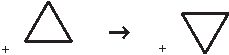
\includegraphics[width=1\textwidth,height=\textheight]{source/figures/shape_grammar_rule.pdf}
\caption{Örnek biçim grameri kuralı (Stiny, 2006).
\label{shapegrammarrule}}
\end{figure}

Biçim gramerleri görsel-mekansal düşünmeyi temsil eden bir biçimcilik
olarakta tanımlanabilmektedir. Görsel tasarım gramerleri olarakta
adlandırabileceğimiz biçim gramerleri dünyaya öğrenilen veya dayatılan
ayrıştırma-tanımlamalar yerine belirli bir zamanda pratik bir anlamı
olan ayrıştırmalardan-tanımlamalardan bakabilme
düşüncesidir-\textbf{yöntemidir} (Özkar ve Stiny, 2009).

Tanıtımından sonra \emph{Gips} (1975) doktora tezinde biçim
gramerlerinin bilgisayar uygulamalarını geliştirdi, \emph{Stiny} (1975)
ise matematiksel temelleri üzerine yoğunlaştı. \emph{Stiny} (1976)
tezinin ardından yazdığı \emph{Two exercises in formal composition} adlı
makalede biçim gramerlerinin kullanımını iki örnek üzerinden açıkladı ve
bu örnekler daha sonra yapılan çalışmalara temel oluşturdu. Bu
örneklerden ilki biçim gramerlerinin üretken bir sistem olarak yeni
tasarım dili veya tarzı oluşturmak için özgün hali ile nasıl
kullanılabildiğini açıklarken ikinci örnek ise mevcut bir tasarım
dilinin veya tarzının biçim gramerleri kullanılarak analizinin nasıl
yapılabildiğini göstermektedir. Ayrıca hem analitik hem de sentetik
kullanıldığı örneklere de rastlamak mümkündür (Knight, 1999).

\hypertarget{analiz-aracux131-olarak-kullanux131mux131-analiz-gramerleri}{%
\subsection{Analiz Aracı Olarak Kullanımı (Analiz
Gramerleri)}\label{analiz-aracux131-olarak-kullanux131mux131-analiz-gramerleri}}

Biçim gramerlerinin ilk kez analiz aracı olarak kullanımı \emph{Stiny}
(1977) tarafından Çin buz ışını pencere tasarımları üzerine yaptığı
çalışmada ortaya konuldu. Bu çalışma ayrıca biçim gramerlerinin
parametrik tasarım ile entegre edilerek parametrik biçim gramerlerinin
tanımlandığı çalışma oldu. Beş adet kuraldan oluşan gramer Çin buz ışını
ızgaraların bir araya gelme düzenini açıklamayı, örnek ızgaralar
oluşturmayı ve sayısız yeni ızgara düzenleri oluşturmayı başardı. Ertesi
yıl \emph{Stiny} ve \emph{Mitchell} (1978) biçim gramerlerini
\emph{Pallodio} stili üzerinden test ederek ilk kez bir mimari üslubun
analizinde kullandılar. ``Palladio Grameri'' kurallarını \emph{Andrea
Palladio} tarafından 1570 yılında yazılmış \emph{Quattro Libri
dell'Architettura}'da bulunan villa planı örneklerini inceleyerek
tanımladılar. Parametrik biçim gramerlerini kullanarak villaların zemin
kat planlarını önerdikleri sekiz aşamalı bir süreç ile oluşturdular.

Bu çalışmanın ardından gelen yirmi yıllık bir dönemde biçim gramerleri
neredeyse tamamen bir analiz aracı olarak mimarların tarzını, yöresel
mimariyi, sanat stillerini vb. açıklamada kullanıldı.

Bu çalışmalar arasında \emph{Giuseppe Terragni}, \emph{Frank Lloyd
Wright}, \emph{Glenn Murcutt}, \emph{Christopher Wren} gibi mimarların
tarzları analiz edildi (Flemming, 1981; Koning ve Eizenberg, 1981;
Hanson ve Radford, 1986; Buelinckx, 1993).

Yöresel mimari analizlerine bakıldığında Japon çay odaları, Buffalo'nun
bungalovları, Queen Anne evleri, geleneksel Tayvan evleri, geleneksel
Türk evleri, sıra evler, klasik Osmanlı dönemi camileri ve Mughul
bahçelerinin peyzaj mimarisi çalışmaları bulunmaktadır (Knight, 1981;
Downing ve Flemming, 1981; Flemming, 1987; Chiou ve Krishnamurti, 1995;
Çağdaş, 1996; Çağdaş, 1996; Aksoy, 2001; Stiny ve Mitchell, 1980).

Sanat stillerinin analizini yapan çalışmalarda \emph{Richard
Diebenkorn}, \emph{Georges Vantongerloo} ve \emph{Fritz Glarner}'ın
tabloları, \emph{Hepplewhite} tarzı sandalyelerin arkalıklarının
tasarımı, \emph{Frank Lloyd Wright}'ın pencere tasarımları ve antik
Yunan çömleklerinin süsleme tasarımları incelenmiştir (Kirsch ve Kirsch,
1986; Knight, 1989; Knight, 1980; Rollo, 1995; Knight, 1986).
\emph{Wright}'ın mimari tarzı için hazırlanan gramer ilk üç boyutlu
mimari gramer çalışması olması açısından önemlidir.

Sonraki dönem çalışmalarında Benros vd. üç ayrı tarz olan Pallodio
villaları, Malagueira konutları ve Prairie konutlarını oluşturdukları
tek gramer, Osmanlı camilerinin ontolojisini kullanan tipolojik
tanımlama (description) gramerleri ve tipolojik tanımlama gramerleri
için genel gösterim önerisi göze çarpmaktadır (Benrós vd., 2014; Stouffs
ve Tunçer, 2015; Stouffs, 2016).

\hypertarget{tasarux131m-aracux131-olarak-kullanux131mux131-uxf6zguxfcn-gramerler}{%
\subsection{Tasarım Aracı Olarak Kullanımı (Özgün
Gramerler)}\label{tasarux131m-aracux131-olarak-kullanux131mux131-uxf6zguxfcn-gramerler}}

Biçim gramerlerinin analiz aracı olarak kullanımı yukarıdaki örneklere
bakıldığında önemli ölçüde etkin olduğunu göstermektedir. Buna karşı
başlangıçtan itibaren tamamen yeni tasarım dilleri oluşturma konusunda
şaşırtıcı bir şekilde sınırlı sayıda örneğe rastlanmaktadır. Bu anlamda
ilk çalışma \emph{Stiny} ve \emph{Gips} (1972) tarafından tablolar
üzerine yapılan biçim gramerleri oldu. \emph{Stiny} ve \emph{Gips}'in
tezleri ve beraber yazdıkları \emph{Algorithmic Aesthetics} kitabı da
yine aynı konu üzerinde biçim grameri formalizmini örnekliyordu (Knight,
1999).

Bu çalışmalar haricinde \emph{Stiny}'nin (1976) iki boyutlu formal
kompozisyonlar ve ilk üç boyutlu biçim grameri çalışması olan Froebel'in
yapı blokları üzerine çalışmaları örnek oluşturmaktadır (Stiny, 1980).
Froebel yapı blokları üzerine olan çalışma özgün gramerleri kullanarak
sıfırdan yeni bir tasarım dili oluşturmak için izlenecek işleyişi
tanımlamaktadır. Yeni tasarım dilini oluşturmak için önerilen işleyişte
biçim sözlüğü, mekansal ilişkiler, biçim kuralları, başlangıç biçimi ve
biçim gramerlerinin aşamalı olarak oluşturulması gerekmektedir. Bu
alanda mimarlık ve diğer dallarda çeşitli çalışmalar kısıtlı sayıda
gerçekleştirildi (Knight, 1989; Knight, 1992; Knight, 1993; Knight,
1994).

\hypertarget{analiz-sonucu-tasarux131m-aracux131-olarak-kullanux131mux131-hibrid-gramerler}{%
\subsection{Analiz Sonucu Tasarım Aracı Olarak Kullanımı (Hibrid
Gramerler)}\label{analiz-sonucu-tasarux131m-aracux131-olarak-kullanux131mux131-hibrid-gramerler}}

Özgün gramelerin tamamen baştan oluşturulması teori üzerinde olmaktadır
(Knight, 1999). Uygulamada ise yeni tasarım dilleri eski ve güncel
dillerin değiştirilmesi, geliştirilmesi veya birleştirmesi gibi işlemler
ile oluşturulur. Knight (1981) önerdiği mevcut tasarım dilleri üzerinden
yeni tasarım dilleri üretme yönteminde ilk önce mevcut dil için bir
gramer çıkartılarak analiz edilir, çıkarılan gramerin kuralları
dönüştürülür ve dönüştürülen kurallar yeni bir gramerin ve dilin temeli
haline gelir. Knight bu yöntemin bilinen dillerin tarihsel evrimini
başarılı bir şekilde tanımlamak ve yeni tasarımlar geliştirmek için
kullanabileceğini belirtmektedir. Bu nedenle bu yöntem hem analitik hem
sentetiktir. Knight \emph{Transformations in Design} adlı kitabında bu
yöntemi kullanarak Frank Lloyd Wright'ın çalışmalarında, De Stijl
resminde ve antik Yunan süsleme tasarımlarında stilistik değişimleri
analiz etmek için uygulamaktadır (Knight, 1999). Flemming (1990)
Knight'ın yöntemine benzer bir yöntemi bilgisayar üzerinde mimari
kompozisyonları öğretebilmek için kullanmmıştır.

Bu gramer yapısının örneklerine baktığımızda Çolakoğlu (2001) 18. ve 19.
yüzyılda Saraybosna'da Osmanlı tarzında tasarlanan geleneksel ``Hayat''
evlerinin gramerini oluşturarak tarihi bağlama uygun yeni formların
üretimini sağladı. Duarte (Duarte, 2005) 1977 ve 1996 yılları arasında
Siza tarafından Malagueira için tasarlanmış otuzbeş konut üzerinden
Siza'nın da desteğini alarak oluşturduğu gramer ile Siza'nın tasarım
mantığına yatkın çeşitli yeni tasarımlar üretebildi. Marakeş Medine'de
\emph{Zaouiat Lakhdar} bölgesi için geliştirilen yerel konut ve kentsel
form üreten gramerler, \emph{rabo-de-bacalhau} bina tipolojisindeki
evlerin rehabilitasyonu için geliştirilen dönüşüm grameri hibrid
gramerlere örnek oluşturmaktadır (Duarte ve Rocha, 2006; Duarte vd.,
2007; Eloy ve Duarte, 2014).

\hypertarget{split-grameri}{%
\subsection{Split Grameri}\label{split-grameri}}

Wonka vd. (2003) mimari modelleri oluşturmak için özel bir set grameri
olan parametrik split gramer yöntemini geliştirmişlerdir. Yazarlar
yapıların yatayda ve düşeyde sürekliliğe sahip olan yapı elemanlarından
oluştuğunu ve buna benzer bir etkiyi split grameri kontrol ederek elde
edilebileceğini belirtmişlerdir. İsmini bölümleme işleminden alan ve iki
üretim kuralı olan bu yöntem basit geometrilerden oluşan üç boyutlu bir
kütlenin önce yüzeylere ve yapısal elemanlarına kadar bölümlenip
ardından bölümlenen her biçim önceden tanımlanan geometri ve malzemeler
ile yer değiştirmesine dayanmaktadır (Şekil \ref{splitGrammar}).
Bölümlenme işlemi sonlandırıcı tanımlı biçimlere ulaşana kadar devam
etmektedir ve muhtemel düzeni önceden tanımlı-sabit olduğundan dolayı
kararlıdır.

Set grameri üretim kurallarını görsel işlem yerine etiketli biçimler
üzerinden işleyen, biçim gramerlerinin basitleştirilmiş halidir (Stiny,
1982; Lienhard, 2017). Etiketli bir biçim set gramerinin en küçük
(atomik) öğesidir ve alt biçimler barındırmaz. Etiketler sembol olarak
kullanılarak üretim kurallarının metinsel olarak yazımını ve
bilgisayarda algoritma olarak işlenmesine olanak vermektedir. İdeal
olarak, bir biçim grameri uygulaması: görsel bilgi işlemeyi
desteklemeli, saklı şekillere (emergence) izin vermeli, önceden
tanımlanmış parçalara dayanmamalı ve parametrik olmalıdır (Gips, 1999).
Set gramerleri biçim gramerlerinin bilgisayar üzerinde işlenmesini
kısıtlayan ilk üç özelliğini barındırmamaktadır. Literatürde biçim
grameri uygulaması olarak adlandırılan bir çok yazılım ve yazılım
denemesi aslında set gramerini temel alarak çalışmaktadır.

\begin{figure}
\centering
\includegraphics[width=0.5\textwidth,height=\textheight]{source/figures/splitGrammar.jpg}
\caption{Basit bir Split Gramer kuralı ve üretim süreci (Sönmez, 2018).
\label{splitGrammar}}
\end{figure}

\begin{figure}
\centering
\includegraphics[width=0.5\textwidth,height=\textheight]{source/figures/splitGrammar2.jpg}
\caption{Bir cephenin katman detay gösterimi (Sönmez, 2018).}
\end{figure}

\hypertarget{cga-biuxe7im-grameri}{%
\subsection{CGA Biçim Grameri}\label{cga-biuxe7im-grameri}}

Split gramerler Müller vd. (2006) tarafından geliştirilerek CGA
gramerleri olarak adlandırılmıştır. Geliştirilen bu yöntemde katı kütle
modelleme sistemi ve farklı olarak tanımlanmış birçok modelleme
kuralının yanında cephe üretimi zor olan karmaşık kütleler içinde
eklentiler bulunmaktadır. CGA gramer yöntemi çokgen ile belirlenmiş bir
parsel hattını yükseltip katlara bölünmüş bir hacim oluşturarak işleme
başlamaktadır. Katların cepheleri biçim kuralları kullanılarak duvar,
kapı, pencere gibi bölümlere bölünmektedir. Koşullu ya da tahmini
kurallar, biçim parametreleri, rastgele numara üretimi bu yöntem
içerisinde çeşitlilik oluşturmak için kullanılmaktadır. CGA bir biçim
grameri olması ile beraber aynı zamanda bir programlama dilidir. Örnek
bir CGA biçim kuralı aşağıdaki gibi yazılmaktadır.

\begin{verbatim}
başlangıçŞekli -->
                    koşul1: sonuçŞekil0 ... sonuçŞekilM ...
                    koşulN: ...
\end{verbatim}

CGA gramerlerinin tanımlanmasının ardından yordamsal modellemenin
kolaylaştırılması ve daha iyi kullanılabilmesi için devamlı gelişmeler
gözlendi. Özellikle cephe modelleri oluşturmak için Müller vd. (2007)
binaların cephe fotoğrafları üzerinden tekrar eden karoların
tanımlanması ile gramer kurallarınının bilgisayar tarafından otomatik
çıkarılması için bir yöntem geliştirdi. Lipp vd. (2008) CGA kurallarını
kod yazarak oluşturmak yerine yaptıkları yazılım sayesinde üç boyutlu
model üzerinden etkileşim ile kodları görsel olarak düzenlemeyi
başardılar. Ancak bu gelişmelere rağmen birçok yordamsal modelleme
projesi kod yazılarak gerçekleştirildi. Bunlardan bazıları;

\begin{itemize}
\tightlist
\item
  Reconstruction of Puuc Buildings (Müller vd., 2006)
\item
  Reconstruction of Ancient Pompeii (Müller vd., 2005)
\item
  Rome Reborn 2.0: A Case Study of Virtual City Reconstruction Using
  Procedural Modeling Techniques (Dylla vd., 2010)
\item
  Urban Topography of Magnesia on the Maeander (Saldaña, 2015).
\end{itemize}

(Zhu, 2017)

(Jesus vd., ) Related work kısmı

\hypertarget{ortahisarux131n-genel-karakteri}{%
\section{Ortahisar'ın Genel
Karakteri}\label{ortahisarux131n-genel-karakteri}}

Zağnos ve Tabakhane vadileri arasında kalan plato üzerine kurulu olan
Ortahisar, Trabzon kentinin en eski yerleşimi olarak surlar tarafından
çevrilmiş şekilde

``Orta - İç Kale'' yerleşkesi

Kentin mimar yapı kültürü M.Ö. 7. yy.a kadar dayanmaktadır.

\begin{figure}
\centering
\includegraphics[width=1\textwidth,height=\textheight]{source/figures/TrabzonMap.png}
\caption{TrabzonMap}
\end{figure}

\hypertarget{konum-ve-ulaux15fux131m}{%
\subsection{Konum ve Ulaşım}\label{konum-ve-ulaux15fux131m}}

\hypertarget{tarihi-ve-karakteri}{%
\subsection{Tarihi ve Karakteri}\label{tarihi-ve-karakteri}}

\hypertarget{bulgular-ve-irdelemeler}{%
\chapter{BULGULAR VE İRDELEMELER}\label{bulgular-ve-irdelemeler}}

\thispagestyle{empty}

\hypertarget{ortahisarux131n-mimari-dil-analizi-ve-biuxe7im-grameri}{%
\section{Ortahisar'ın Mimari Dil Analizi ve Biçim
Grameri}\label{ortahisarux131n-mimari-dil-analizi-ve-biuxe7im-grameri}}

\hypertarget{yapux131-taban-alanux131-analizi}{%
\subsection{Yapı Taban Alanı
Analizi}\label{yapux131-taban-alanux131-analizi}}

Seçilen Ortahisar evlerinin taban alanları, derinlikleri, genişlikleri
incelendiğinde

\begin{itemize}
\tightlist
\item
  En küçük yapı taban alanı : 50,38 m\textsuperscript{2}
\item
  En büyük yapı taban alanı : 315,67 m\textsuperscript{2}
\item
  En kısa kenar uzunluğu : 4,888 m
\item
  En uzun kenar uzunluğu : 17,021 m
\item
  Plan derinliğinin genişliğine oranının en küçük değeri 0,346 en büyük
  değeri 1,513
\end{itemize}

oldukları bulunmuştur.

\begin{longtable}[]{@{}rrrrrrr@{}}
\caption{Seçilmiş Ortahisar evlerinin oturum alanları, ortalama derinlik
ve ortalama genişlik değerleri tablosu.
\label{EvlerAlanlarOrtalamalar}}\tabularnewline
\toprule
\textbf{Ada} & \textbf{Parsel} & \textbf{Ort. Derinlik} & \textbf{Ort.
Genişlik} & \textbf{Der. / Gen.} & \textbf{Taban Alanı} & \textbf{Parsel
Alanı}\tabularnewline
\midrule
\endfirsthead
\toprule
\textbf{Ada} & \textbf{Parsel} & \textbf{Ort. Derinlik} & \textbf{Ort.
Genişlik} & \textbf{Der. / Gen.} & \textbf{Taban Alanı} & \textbf{Parsel
Alanı}\tabularnewline
\midrule
\endhead
\textbf{110} & \textbf{16} & 7,955 m & 12,628 m & 0,630 & 100,43
m\textsuperscript{2} & 191,09 m\textsuperscript{2}\tabularnewline
\textbf{110} & \textbf{23} & 5,012 m & 10,067 m & 0,498 & 50,38
m\textsuperscript{2} & 84,07 m\textsuperscript{2}\tabularnewline
\textbf{110} & \textbf{39} & 12,678 m & 16,048 m & 0,790 & 194,83
m\textsuperscript{2} & 890,45 m\textsuperscript{2}\tabularnewline
\textbf{110} & \textbf{41} & 8,528 m & 14,385 m & 0,593 & 117,90
m\textsuperscript{2} & 320,49 m\textsuperscript{2}\tabularnewline
\textbf{110} & \textbf{43} & 12,501 m & 8,320 m & 1,503 & 110,31
m\textsuperscript{2} & 124,59 m\textsuperscript{2}\tabularnewline
\textbf{110} & \textbf{44} & 10,284 m & 8,165 m & 1,259 & 74,16
m\textsuperscript{2} & 45,80 m\textsuperscript{2}\tabularnewline
\textbf{110} & \textbf{131} & 6,670 m & 13,247 m & 0,503 & 93,91
m\textsuperscript{2} & 1.639,41 m\textsuperscript{2}\tabularnewline
\textbf{114} & \textbf{30} & 10,975 m & 7,255 m & 1,513 & 100,23
m\textsuperscript{2} & 131,28 m\textsuperscript{2}\tabularnewline
\textbf{118} & \textbf{1} & 9,208 m & 14,904 m & 0,618 & 137,30
m\textsuperscript{2} & 177,17 m\textsuperscript{2}\tabularnewline
\textbf{127} & \textbf{12} & 9,706 m & 11,437 m & 0,849 & 87,50
m\textsuperscript{2} & 318,80 m\textsuperscript{2}\tabularnewline
\textbf{127} & \textbf{28} & 8,473 m & 9,799 m & 0,865 & 83,43
m\textsuperscript{2} & 205,86 m\textsuperscript{2}\tabularnewline
\textbf{128} & \textbf{7} & 8,473 m & 10,102 m & 0,839 & 92,20
m\textsuperscript{2} & 180,38 m\textsuperscript{2}\tabularnewline
\textbf{128} & \textbf{10} & 4,888 m & 14,111 m & 0,346 & 61,41
m\textsuperscript{2} & 102,06 m\textsuperscript{2}\tabularnewline
\textbf{129} & \textbf{26} & 16,493 m & 15,992 m & 1,031 & 242,79
m\textsuperscript{2} & 203,24 m\textsuperscript{2}\tabularnewline
\textbf{888} & \textbf{7} & 15,746 m & 12,945 m & 1,216 & 199,34
m\textsuperscript{2} & 603,81 m\textsuperscript{2}\tabularnewline
\textbf{888} & \textbf{8} & 14,998 m & 17,021 m & 0,881 & 315,67
m\textsuperscript{2} & 879,21 m\textsuperscript{2}\tabularnewline
\bottomrule
\end{longtable}

\hypertarget{yapux131-kat-sayux131sux131-ve-yuxfckseklikleri-analizi}{%
\subsection{Yapı Kat Sayısı ve Yükseklikleri
Analizi}\label{yapux131-kat-sayux131sux131-ve-yuxfckseklikleri-analizi}}

\begin{figure}
\centering
\includegraphics[width=1\textwidth,height=\textheight]{source/figures/katgruplandirma.pdf}
\caption{Ortahisar evlerinin kat sayısına göre gruplandırılması.
\label{katgruplama}}
\end{figure}

\begin{longtable}[]{@{}rrrrrrr@{}}
\caption{Kat yükseklikleri tablosu.}\tabularnewline
\toprule
\textbf{Ada} & \textbf{Parsel} & \textbf{Bodrum Kat} & \textbf{Zemin
Kat} & \textbf{Birinci Kat} & \textbf{İkinci Kat} & \textbf{Çatı
Katı}\tabularnewline
\midrule
\endfirsthead
\toprule
\textbf{Ada} & \textbf{Parsel} & \textbf{Bodrum Kat} & \textbf{Zemin
Kat} & \textbf{Birinci Kat} & \textbf{İkinci Kat} & \textbf{Çatı
Katı}\tabularnewline
\midrule
\endhead
\textbf{118} & \textbf{1} & 2,369 m & 3,733 m & 3,318 m & 3,760 m
&\tabularnewline
\textbf{128} & \textbf{10} & 2,441 m & 4,046 m & 3,247 m & 3,239 m
&\tabularnewline
\textbf{110} & \textbf{16} & 3,242 m & 3,706 m & 4,021 m & & 3,325
m\tabularnewline
\textbf{110} & \textbf{39} & 1,935 m & 4,180 m & 4,093 m & & 2,402
m\tabularnewline
\textbf{110} & \textbf{41} & 1,823 m & 3,693 m & 4,083 m & & 2,334
m\tabularnewline
\textbf{110} & \textbf{131} & & 2,766 m & 3,229 m & 3,348 m & 2,547
m\tabularnewline
\textbf{129} & \textbf{26} & 2,002 m & 3,443 m & 3,226 m & & 3,258
m\tabularnewline
\textbf{110} & \textbf{44} & 2,783 m & 4,663 m & 2,933 m & 2,913 m
&\tabularnewline
\textbf{114} & \textbf{30} & 2,946 m & 3,524 m & 3,252 m &
&\tabularnewline
\textbf{128} & \textbf{7} & 2,431 m & 4,057 m & 3,807 m &
&\tabularnewline
\textbf{888} & \textbf{8} & & 4,227 m & 4,065 m & 4,595 m
&\tabularnewline
\textbf{127} & \textbf{28} & & 2,897 m & 3,840 m & & 2,871
m\tabularnewline
\textbf{110} & \textbf{23} & 1,752 m & 3,112 m & 3,189 m &
&\tabularnewline
\textbf{110} & \textbf{43} & & 4,305 m & 4,147 m & &\tabularnewline
\textbf{127} & \textbf{12} & 1,086 m & 3,288 m & 3,635 m &
&\tabularnewline
\textbf{888} & \textbf{7} & & 4,682 m & 3,828 m & &\tabularnewline
\bottomrule
\end{longtable}

\begin{longtable}[]{@{}lrrrrrrr@{}}
\caption{Kat sayısına göre gruplandırılmış kat oranları
tablosu.}\tabularnewline
\toprule
\begin{minipage}[b]{0.02\columnwidth}\raggedright
\strut
\end{minipage} & \begin{minipage}[b]{0.04\columnwidth}\raggedleft
\textbf{Ada}\strut
\end{minipage} & \begin{minipage}[b]{0.04\columnwidth}\raggedleft
\textbf{Parsel}\strut
\end{minipage} & \begin{minipage}[b]{0.14\columnwidth}\raggedleft
\textbf{Zemin Kat}\strut
\end{minipage} & \begin{minipage}[b]{0.14\columnwidth}\raggedleft
\textbf{Bodrum K. / Zemin K.}\strut
\end{minipage} & \begin{minipage}[b]{0.14\columnwidth}\raggedleft
\textbf{Birinci K. / Zemin K.}\strut
\end{minipage} & \begin{minipage}[b]{0.14\columnwidth}\raggedleft
\textbf{İkinci K. / Zemin K.}\strut
\end{minipage} & \begin{minipage}[b]{0.12\columnwidth}\raggedleft
\textbf{Çatı K. / Zemin K.}\strut
\end{minipage}\tabularnewline
\midrule
\endfirsthead
\toprule
\begin{minipage}[b]{0.02\columnwidth}\raggedright
\strut
\end{minipage} & \begin{minipage}[b]{0.04\columnwidth}\raggedleft
\textbf{Ada}\strut
\end{minipage} & \begin{minipage}[b]{0.04\columnwidth}\raggedleft
\textbf{Parsel}\strut
\end{minipage} & \begin{minipage}[b]{0.14\columnwidth}\raggedleft
\textbf{Zemin Kat}\strut
\end{minipage} & \begin{minipage}[b]{0.14\columnwidth}\raggedleft
\textbf{Bodrum K. / Zemin K.}\strut
\end{minipage} & \begin{minipage}[b]{0.14\columnwidth}\raggedleft
\textbf{Birinci K. / Zemin K.}\strut
\end{minipage} & \begin{minipage}[b]{0.14\columnwidth}\raggedleft
\textbf{İkinci K. / Zemin K.}\strut
\end{minipage} & \begin{minipage}[b]{0.12\columnwidth}\raggedleft
\textbf{Çatı K. / Zemin K.}\strut
\end{minipage}\tabularnewline
\midrule
\endhead
\begin{minipage}[t]{0.02\columnwidth}\raggedright
\textbf{4}\strut
\end{minipage} & \begin{minipage}[t]{0.04\columnwidth}\raggedleft
\strut
\end{minipage} & \begin{minipage}[t]{0.04\columnwidth}\raggedleft
\strut
\end{minipage} & \begin{minipage}[t]{0.14\columnwidth}\raggedleft
\strut
\end{minipage} & \begin{minipage}[t]{0.14\columnwidth}\raggedleft
\strut
\end{minipage} & \begin{minipage}[t]{0.14\columnwidth}\raggedleft
\strut
\end{minipage} & \begin{minipage}[t]{0.14\columnwidth}\raggedleft
\strut
\end{minipage} & \begin{minipage}[t]{0.12\columnwidth}\raggedleft
\strut
\end{minipage}\tabularnewline
\begin{minipage}[t]{0.02\columnwidth}\raggedright
\strut
\end{minipage} & \begin{minipage}[t]{0.04\columnwidth}\raggedleft
\textbf{118}\strut
\end{minipage} & \begin{minipage}[t]{0.04\columnwidth}\raggedleft
\textbf{1}\strut
\end{minipage} & \begin{minipage}[t]{0.14\columnwidth}\raggedleft
3,733 m\strut
\end{minipage} & \begin{minipage}[t]{0.14\columnwidth}\raggedleft
0,635\strut
\end{minipage} & \begin{minipage}[t]{0.14\columnwidth}\raggedleft
0,889\strut
\end{minipage} & \begin{minipage}[t]{0.14\columnwidth}\raggedleft
1,007\strut
\end{minipage} & \begin{minipage}[t]{0.12\columnwidth}\raggedleft
\strut
\end{minipage}\tabularnewline
\begin{minipage}[t]{0.02\columnwidth}\raggedright
\strut
\end{minipage} & \begin{minipage}[t]{0.04\columnwidth}\raggedleft
\textbf{128}\strut
\end{minipage} & \begin{minipage}[t]{0.04\columnwidth}\raggedleft
\textbf{10}\strut
\end{minipage} & \begin{minipage}[t]{0.14\columnwidth}\raggedleft
4,046 m\strut
\end{minipage} & \begin{minipage}[t]{0.14\columnwidth}\raggedleft
0,603\strut
\end{minipage} & \begin{minipage}[t]{0.14\columnwidth}\raggedleft
0,802\strut
\end{minipage} & \begin{minipage}[t]{0.14\columnwidth}\raggedleft
0,801\strut
\end{minipage} & \begin{minipage}[t]{0.12\columnwidth}\raggedleft
\strut
\end{minipage}\tabularnewline
\begin{minipage}[t]{0.02\columnwidth}\raggedright
\textbf{3,5}\strut
\end{minipage} & \begin{minipage}[t]{0.04\columnwidth}\raggedleft
\strut
\end{minipage} & \begin{minipage}[t]{0.04\columnwidth}\raggedleft
\strut
\end{minipage} & \begin{minipage}[t]{0.14\columnwidth}\raggedleft
\strut
\end{minipage} & \begin{minipage}[t]{0.14\columnwidth}\raggedleft
\strut
\end{minipage} & \begin{minipage}[t]{0.14\columnwidth}\raggedleft
\strut
\end{minipage} & \begin{minipage}[t]{0.14\columnwidth}\raggedleft
\strut
\end{minipage} & \begin{minipage}[t]{0.12\columnwidth}\raggedleft
\strut
\end{minipage}\tabularnewline
\begin{minipage}[t]{0.02\columnwidth}\raggedright
\strut
\end{minipage} & \begin{minipage}[t]{0.04\columnwidth}\raggedleft
\textbf{110}\strut
\end{minipage} & \begin{minipage}[t]{0.04\columnwidth}\raggedleft
\textbf{16}\strut
\end{minipage} & \begin{minipage}[t]{0.14\columnwidth}\raggedleft
3,706 m\strut
\end{minipage} & \begin{minipage}[t]{0.14\columnwidth}\raggedleft
0,875\strut
\end{minipage} & \begin{minipage}[t]{0.14\columnwidth}\raggedleft
1,085\strut
\end{minipage} & \begin{minipage}[t]{0.14\columnwidth}\raggedleft
\strut
\end{minipage} & \begin{minipage}[t]{0.12\columnwidth}\raggedleft
0,897\strut
\end{minipage}\tabularnewline
\begin{minipage}[t]{0.02\columnwidth}\raggedright
\strut
\end{minipage} & \begin{minipage}[t]{0.04\columnwidth}\raggedleft
\textbf{110}\strut
\end{minipage} & \begin{minipage}[t]{0.04\columnwidth}\raggedleft
\textbf{39}\strut
\end{minipage} & \begin{minipage}[t]{0.14\columnwidth}\raggedleft
4,180 m\strut
\end{minipage} & \begin{minipage}[t]{0.14\columnwidth}\raggedleft
0,463\strut
\end{minipage} & \begin{minipage}[t]{0.14\columnwidth}\raggedleft
0,979\strut
\end{minipage} & \begin{minipage}[t]{0.14\columnwidth}\raggedleft
\strut
\end{minipage} & \begin{minipage}[t]{0.12\columnwidth}\raggedleft
0,575\strut
\end{minipage}\tabularnewline
\begin{minipage}[t]{0.02\columnwidth}\raggedright
\strut
\end{minipage} & \begin{minipage}[t]{0.04\columnwidth}\raggedleft
\textbf{110}\strut
\end{minipage} & \begin{minipage}[t]{0.04\columnwidth}\raggedleft
\textbf{41}\strut
\end{minipage} & \begin{minipage}[t]{0.14\columnwidth}\raggedleft
3,693 m\strut
\end{minipage} & \begin{minipage}[t]{0.14\columnwidth}\raggedleft
0,494\strut
\end{minipage} & \begin{minipage}[t]{0.14\columnwidth}\raggedleft
1,106\strut
\end{minipage} & \begin{minipage}[t]{0.14\columnwidth}\raggedleft
\strut
\end{minipage} & \begin{minipage}[t]{0.12\columnwidth}\raggedleft
0,632\strut
\end{minipage}\tabularnewline
\begin{minipage}[t]{0.02\columnwidth}\raggedright
\strut
\end{minipage} & \begin{minipage}[t]{0.04\columnwidth}\raggedleft
\textbf{110}\strut
\end{minipage} & \begin{minipage}[t]{0.04\columnwidth}\raggedleft
\textbf{131}\strut
\end{minipage} & \begin{minipage}[t]{0.14\columnwidth}\raggedleft
2,766 m\strut
\end{minipage} & \begin{minipage}[t]{0.14\columnwidth}\raggedleft
\strut
\end{minipage} & \begin{minipage}[t]{0.14\columnwidth}\raggedleft
1,167\strut
\end{minipage} & \begin{minipage}[t]{0.14\columnwidth}\raggedleft
1,210\strut
\end{minipage} & \begin{minipage}[t]{0.12\columnwidth}\raggedleft
0,921\strut
\end{minipage}\tabularnewline
\begin{minipage}[t]{0.02\columnwidth}\raggedright
\strut
\end{minipage} & \begin{minipage}[t]{0.04\columnwidth}\raggedleft
\textbf{129}\strut
\end{minipage} & \begin{minipage}[t]{0.04\columnwidth}\raggedleft
\textbf{26}\strut
\end{minipage} & \begin{minipage}[t]{0.14\columnwidth}\raggedleft
3,443 m\strut
\end{minipage} & \begin{minipage}[t]{0.14\columnwidth}\raggedleft
0,581\strut
\end{minipage} & \begin{minipage}[t]{0.14\columnwidth}\raggedleft
0,937\strut
\end{minipage} & \begin{minipage}[t]{0.14\columnwidth}\raggedleft
\strut
\end{minipage} & \begin{minipage}[t]{0.12\columnwidth}\raggedleft
0,946\strut
\end{minipage}\tabularnewline
\begin{minipage}[t]{0.02\columnwidth}\raggedright
\textbf{3}\strut
\end{minipage} & \begin{minipage}[t]{0.04\columnwidth}\raggedleft
\strut
\end{minipage} & \begin{minipage}[t]{0.04\columnwidth}\raggedleft
\strut
\end{minipage} & \begin{minipage}[t]{0.14\columnwidth}\raggedleft
\strut
\end{minipage} & \begin{minipage}[t]{0.14\columnwidth}\raggedleft
\strut
\end{minipage} & \begin{minipage}[t]{0.14\columnwidth}\raggedleft
\strut
\end{minipage} & \begin{minipage}[t]{0.14\columnwidth}\raggedleft
\strut
\end{minipage} & \begin{minipage}[t]{0.12\columnwidth}\raggedleft
\strut
\end{minipage}\tabularnewline
\begin{minipage}[t]{0.02\columnwidth}\raggedright
\strut
\end{minipage} & \begin{minipage}[t]{0.04\columnwidth}\raggedleft
\textbf{110}\strut
\end{minipage} & \begin{minipage}[t]{0.04\columnwidth}\raggedleft
\textbf{44}\strut
\end{minipage} & \begin{minipage}[t]{0.14\columnwidth}\raggedleft
4,663 m\strut
\end{minipage} & \begin{minipage}[t]{0.14\columnwidth}\raggedleft
\strut
\end{minipage} & \begin{minipage}[t]{0.14\columnwidth}\raggedleft
0,629\strut
\end{minipage} & \begin{minipage}[t]{0.14\columnwidth}\raggedleft
0,625\strut
\end{minipage} & \begin{minipage}[t]{0.12\columnwidth}\raggedleft
\strut
\end{minipage}\tabularnewline
\begin{minipage}[t]{0.02\columnwidth}\raggedright
\strut
\end{minipage} & \begin{minipage}[t]{0.04\columnwidth}\raggedleft
\textbf{114}\strut
\end{minipage} & \begin{minipage}[t]{0.04\columnwidth}\raggedleft
\textbf{30}\strut
\end{minipage} & \begin{minipage}[t]{0.14\columnwidth}\raggedleft
3,524 m\strut
\end{minipage} & \begin{minipage}[t]{0.14\columnwidth}\raggedleft
0,836\strut
\end{minipage} & \begin{minipage}[t]{0.14\columnwidth}\raggedleft
0,923\strut
\end{minipage} & \begin{minipage}[t]{0.14\columnwidth}\raggedleft
\strut
\end{minipage} & \begin{minipage}[t]{0.12\columnwidth}\raggedleft
\strut
\end{minipage}\tabularnewline
\begin{minipage}[t]{0.02\columnwidth}\raggedright
\strut
\end{minipage} & \begin{minipage}[t]{0.04\columnwidth}\raggedleft
\textbf{128}\strut
\end{minipage} & \begin{minipage}[t]{0.04\columnwidth}\raggedleft
\textbf{7}\strut
\end{minipage} & \begin{minipage}[t]{0.14\columnwidth}\raggedleft
4,057 m\strut
\end{minipage} & \begin{minipage}[t]{0.14\columnwidth}\raggedleft
0,599\strut
\end{minipage} & \begin{minipage}[t]{0.14\columnwidth}\raggedleft
0,938\strut
\end{minipage} & \begin{minipage}[t]{0.14\columnwidth}\raggedleft
\strut
\end{minipage} & \begin{minipage}[t]{0.12\columnwidth}\raggedleft
\strut
\end{minipage}\tabularnewline
\begin{minipage}[t]{0.02\columnwidth}\raggedright
\strut
\end{minipage} & \begin{minipage}[t]{0.04\columnwidth}\raggedleft
\textbf{888}\strut
\end{minipage} & \begin{minipage}[t]{0.04\columnwidth}\raggedleft
\textbf{8}\strut
\end{minipage} & \begin{minipage}[t]{0.14\columnwidth}\raggedleft
4,227 m\strut
\end{minipage} & \begin{minipage}[t]{0.14\columnwidth}\raggedleft
\strut
\end{minipage} & \begin{minipage}[t]{0.14\columnwidth}\raggedleft
0,962\strut
\end{minipage} & \begin{minipage}[t]{0.14\columnwidth}\raggedleft
1,087\strut
\end{minipage} & \begin{minipage}[t]{0.12\columnwidth}\raggedleft
\strut
\end{minipage}\tabularnewline
\begin{minipage}[t]{0.02\columnwidth}\raggedright
\textbf{2,5}\strut
\end{minipage} & \begin{minipage}[t]{0.04\columnwidth}\raggedleft
\strut
\end{minipage} & \begin{minipage}[t]{0.04\columnwidth}\raggedleft
\strut
\end{minipage} & \begin{minipage}[t]{0.14\columnwidth}\raggedleft
\strut
\end{minipage} & \begin{minipage}[t]{0.14\columnwidth}\raggedleft
\strut
\end{minipage} & \begin{minipage}[t]{0.14\columnwidth}\raggedleft
\strut
\end{minipage} & \begin{minipage}[t]{0.14\columnwidth}\raggedleft
\strut
\end{minipage} & \begin{minipage}[t]{0.12\columnwidth}\raggedleft
\strut
\end{minipage}\tabularnewline
\begin{minipage}[t]{0.02\columnwidth}\raggedright
\strut
\end{minipage} & \begin{minipage}[t]{0.04\columnwidth}\raggedleft
\textbf{127}\strut
\end{minipage} & \begin{minipage}[t]{0.04\columnwidth}\raggedleft
\textbf{28}\strut
\end{minipage} & \begin{minipage}[t]{0.14\columnwidth}\raggedleft
2,897 m\strut
\end{minipage} & \begin{minipage}[t]{0.14\columnwidth}\raggedleft
\strut
\end{minipage} & \begin{minipage}[t]{0.14\columnwidth}\raggedleft
1,325\strut
\end{minipage} & \begin{minipage}[t]{0.14\columnwidth}\raggedleft
\strut
\end{minipage} & \begin{minipage}[t]{0.12\columnwidth}\raggedleft
0,991\strut
\end{minipage}\tabularnewline
\begin{minipage}[t]{0.02\columnwidth}\raggedright
\textbf{2}\strut
\end{minipage} & \begin{minipage}[t]{0.04\columnwidth}\raggedleft
\strut
\end{minipage} & \begin{minipage}[t]{0.04\columnwidth}\raggedleft
\strut
\end{minipage} & \begin{minipage}[t]{0.14\columnwidth}\raggedleft
\strut
\end{minipage} & \begin{minipage}[t]{0.14\columnwidth}\raggedleft
\strut
\end{minipage} & \begin{minipage}[t]{0.14\columnwidth}\raggedleft
\strut
\end{minipage} & \begin{minipage}[t]{0.14\columnwidth}\raggedleft
\strut
\end{minipage} & \begin{minipage}[t]{0.12\columnwidth}\raggedleft
\strut
\end{minipage}\tabularnewline
\begin{minipage}[t]{0.02\columnwidth}\raggedright
\strut
\end{minipage} & \begin{minipage}[t]{0.04\columnwidth}\raggedleft
\textbf{110}\strut
\end{minipage} & \begin{minipage}[t]{0.04\columnwidth}\raggedleft
\textbf{23}\strut
\end{minipage} & \begin{minipage}[t]{0.14\columnwidth}\raggedleft
3,112 m\strut
\end{minipage} & \begin{minipage}[t]{0.14\columnwidth}\raggedleft
0,563\strut
\end{minipage} & \begin{minipage}[t]{0.14\columnwidth}\raggedleft
1,025\strut
\end{minipage} & \begin{minipage}[t]{0.14\columnwidth}\raggedleft
\strut
\end{minipage} & \begin{minipage}[t]{0.12\columnwidth}\raggedleft
\strut
\end{minipage}\tabularnewline
\begin{minipage}[t]{0.02\columnwidth}\raggedright
\strut
\end{minipage} & \begin{minipage}[t]{0.04\columnwidth}\raggedleft
\textbf{110}\strut
\end{minipage} & \begin{minipage}[t]{0.04\columnwidth}\raggedleft
\textbf{43}\strut
\end{minipage} & \begin{minipage}[t]{0.14\columnwidth}\raggedleft
4,305 m\strut
\end{minipage} & \begin{minipage}[t]{0.14\columnwidth}\raggedleft
\strut
\end{minipage} & \begin{minipage}[t]{0.14\columnwidth}\raggedleft
0,963\strut
\end{minipage} & \begin{minipage}[t]{0.14\columnwidth}\raggedleft
\strut
\end{minipage} & \begin{minipage}[t]{0.12\columnwidth}\raggedleft
\strut
\end{minipage}\tabularnewline
\begin{minipage}[t]{0.02\columnwidth}\raggedright
\strut
\end{minipage} & \begin{minipage}[t]{0.04\columnwidth}\raggedleft
\textbf{127}\strut
\end{minipage} & \begin{minipage}[t]{0.04\columnwidth}\raggedleft
\textbf{12}\strut
\end{minipage} & \begin{minipage}[t]{0.14\columnwidth}\raggedleft
3,288 m\strut
\end{minipage} & \begin{minipage}[t]{0.14\columnwidth}\raggedleft
0,330\strut
\end{minipage} & \begin{minipage}[t]{0.14\columnwidth}\raggedleft
1,105\strut
\end{minipage} & \begin{minipage}[t]{0.14\columnwidth}\raggedleft
\strut
\end{minipage} & \begin{minipage}[t]{0.12\columnwidth}\raggedleft
\strut
\end{minipage}\tabularnewline
\begin{minipage}[t]{0.02\columnwidth}\raggedright
\strut
\end{minipage} & \begin{minipage}[t]{0.04\columnwidth}\raggedleft
\textbf{888}\strut
\end{minipage} & \begin{minipage}[t]{0.04\columnwidth}\raggedleft
\textbf{7}\strut
\end{minipage} & \begin{minipage}[t]{0.14\columnwidth}\raggedleft
4,682 m\strut
\end{minipage} & \begin{minipage}[t]{0.14\columnwidth}\raggedleft
\strut
\end{minipage} & \begin{minipage}[t]{0.14\columnwidth}\raggedleft
0,818\strut
\end{minipage} & \begin{minipage}[t]{0.14\columnwidth}\raggedleft
\strut
\end{minipage} & \begin{minipage}[t]{0.12\columnwidth}\raggedleft
\strut
\end{minipage}\tabularnewline
\bottomrule
\end{longtable}

\newpage

\hypertarget{cephe-analizi}{%
\subsection{Cephe Analizi}\label{cephe-analizi}}

\begin{figure}
\centering
\includegraphics[width=0.85\textwidth,height=\textheight]{source/figures/cephegruplandirma.pdf}
\caption{Ortahisar evlerinin cephe kurgusuna göre gruplandırılması. Sol
tarafta 3 parçalı ve sağ tarafta 1 parçalı cephe düzenleri.
\label{cephegruplama}}
\end{figure}

\newpage

\begin{longtable}[]{@{}lrrrrrrr@{}}
\caption{Ortahisar evlerinin cephe parçalarının genişlik oranları
analizi tablosu.}\tabularnewline
\toprule
& \textbf{Ada} & \textbf{Parsel} & \textbf{Bay Sol} & \textbf{Bay Orta}
& \textbf{Bay Sağ} & \textbf{Sol / Orta} & \textbf{Sağ /
Orta}\tabularnewline
\midrule
\endfirsthead
\toprule
& \textbf{Ada} & \textbf{Parsel} & \textbf{Bay Sol} & \textbf{Bay Orta}
& \textbf{Bay Sağ} & \textbf{Sol / Orta} & \textbf{Sağ /
Orta}\tabularnewline
\midrule
\endhead
\textbf{3 Bay} & & & & & & &\tabularnewline
& \textbf{118} & \textbf{1} & 5,180 m & 4,480 m & 5,220 m & 1,156 &
1,165\tabularnewline
& \textbf{128} & \textbf{10} & 4,580 m & 4,740 m & 4,600 m & 0,966 &
0,970\tabularnewline
& \textbf{110} & \textbf{16} & 4,280 m & 4,710 m & 4,420 m & 0,909 &
0,938\tabularnewline
& \textbf{110} & \textbf{39} & 5,230 m & 4,960 m & 5,320 m & 1,054 &
1,073\tabularnewline
& \textbf{110} & \textbf{41} & 5,360 m & 3,750 m & 5,320 m & 1,429 &
1,419\tabularnewline
& \textbf{110} & \textbf{131} & 4,470 m & 4,090 m & 4,680 m & 1,093 &
1,144\tabularnewline
& \textbf{129} & \textbf{26} & 5,020 m & 5,340 m & 4,960 m & 0,940 &
0,929\tabularnewline
& \textbf{888} & \textbf{8} & 6,420 m & 6,160 m & 6,480 m & 1,042 &
1,052\tabularnewline
& \textbf{127} & \textbf{28} & 3,370 m & 3,110 m & 3,260 m & 1,084 &
1,048\tabularnewline
& \textbf{110} & \textbf{23} & 3,470 m & 2,990 m & 3,600 m & 1,161 &
1,204\tabularnewline
& \textbf{110} & \textbf{43} & 3,960 m & 3,960 m & 3,960 m & 1,000 &
1,000\tabularnewline
& \textbf{888} & \textbf{7} & 5,220 m & 3,550 m & 4,660 m & 1,470 &
1,313\tabularnewline
\textbf{1 Bay} & & & & & & &\tabularnewline
& \textbf{110} & \textbf{44} & 7,160 m & & & &\tabularnewline
& \textbf{114} & \textbf{30} & 8,850 m & & & &\tabularnewline
& \textbf{128} & \textbf{7} & 9,930 m & & & &\tabularnewline
\bottomrule
\end{longtable}

\begin{longtable}[]{@{}lrrrrrr@{}}
\caption{Sol ve sağ cephe parçalarındaki pencere sayılarının
tablosu.}\tabularnewline
\toprule
& \textbf{Ada} & \textbf{Parsel} & \textbf{Zemin Kat} & \textbf{Birinci
Kat} & \textbf{İkinci Kat} & \textbf{Çatı Katı}\tabularnewline
\midrule
\endfirsthead
\toprule
& \textbf{Ada} & \textbf{Parsel} & \textbf{Zemin Kat} & \textbf{Birinci
Kat} & \textbf{İkinci Kat} & \textbf{Çatı Katı}\tabularnewline
\midrule
\endhead
\textbf{3 Bay} & & & & & &\tabularnewline
& \textbf{118} & \textbf{1} & 2 & 3 & 3 &\tabularnewline
& \textbf{128} & \textbf{10} & 1 & 1 & 1 &\tabularnewline
& \textbf{110} & \textbf{16} & 2 & 2 & & 3\tabularnewline
& \textbf{110} & \textbf{39} & 2 & 2 & & 2\tabularnewline
& \textbf{110} & \textbf{41} & 2 & 2 & & 2\tabularnewline
& \textbf{110} & \textbf{131} & 3 & 3 & 3 & 2\tabularnewline
& \textbf{129} & \textbf{26} & 2 & 2 & & 3\tabularnewline
& \textbf{888} & \textbf{8} & 3 & 3 & 3 &\tabularnewline
& \textbf{127} & \textbf{28} & 2 & 1 & & 1\tabularnewline
& \textbf{110} & \textbf{23} & 1 & 1 & &\tabularnewline
& \textbf{110} & \textbf{43} & 1 & 2 & &\tabularnewline
& \textbf{888} & \textbf{7} & 1 & 3 & &\tabularnewline
\bottomrule
\end{longtable}

\begin{longtable}[]{@{}lrrrrrr@{}}
\caption{Orta cephe parçalarındaki pencere sayılarının tablosu. Tek
parçalı cepheye sahip evler bu tabloda gösterilmiştir.}\tabularnewline
\toprule
& \textbf{Ada} & \textbf{Parsel} & \textbf{Zemin Kat} & \textbf{Birinci
Kat} & \textbf{İkinci Kat} & \textbf{Çatı Katı}\tabularnewline
\midrule
\endfirsthead
\toprule
& \textbf{Ada} & \textbf{Parsel} & \textbf{Zemin Kat} & \textbf{Birinci
Kat} & \textbf{İkinci Kat} & \textbf{Çatı Katı}\tabularnewline
\midrule
\endhead
\textbf{3 Bay} & & & & & &\tabularnewline
& \textbf{118} & \textbf{1} & Giriş & 3 & 3 &\tabularnewline
& \textbf{128} & \textbf{10} & Giriş & 1 & 1 &\tabularnewline
& \textbf{110} & \textbf{16} & 2 & 2 & & 3\tabularnewline
& \textbf{110} & \textbf{39} & Giriş & Kapalı balkon & &
2\tabularnewline
& \textbf{110} & \textbf{41} & Giriş & 2 & & 2\tabularnewline
& \textbf{110} & \textbf{131} & Giriş & 2 & 2 & 2\tabularnewline
& \textbf{129} & \textbf{26} & 3 & 3 & & 3\tabularnewline
& \textbf{888} & \textbf{8} & Giriş & 2 & 2 &\tabularnewline
& \textbf{127} & \textbf{28} & Giriş & 2 & & 2\tabularnewline
& \textbf{110} & \textbf{23} & Giriş & 1 & &\tabularnewline
& \textbf{110} & \textbf{43} & 1 & 2 & &\tabularnewline
& \textbf{888} & \textbf{7} & Giriş & 2 & &\tabularnewline
\textbf{1 Bay} & & & & & &\tabularnewline
& \textbf{110} & \textbf{44} & 2 & 5 & 5 &\tabularnewline
& \textbf{114} & \textbf{30} & 6 & 6 & &\tabularnewline
& \textbf{128} & \textbf{7} & 4 & 4 & &\tabularnewline
\bottomrule
\end{longtable}

\newpage

\hypertarget{cephe-uxe7ux131kmalarux131-analizi-cumba}{%
\subsection{Cephe Çıkmaları Analizi
(Cumba)}\label{cephe-uxe7ux131kmalarux131-analizi-cumba}}

\begin{longtable}[]{@{}rrrrrr@{}}
\caption{Cumbaların derinlik ölçüleri tablosu.}\tabularnewline
\toprule
\textbf{Ada} & \textbf{Parsel} & \textbf{Zemin Kat} & \textbf{Birinci
Kat} & \textbf{İkinci Kat} & \textbf{Çatı Katı}\tabularnewline
\midrule
\endfirsthead
\toprule
\textbf{Ada} & \textbf{Parsel} & \textbf{Zemin Kat} & \textbf{Birinci
Kat} & \textbf{İkinci Kat} & \textbf{Çatı Katı}\tabularnewline
\midrule
\endhead
\textbf{118} & \textbf{1} & & 1,900 m & 2,300 m &\tabularnewline
\textbf{128} & \textbf{10} & & 1,460 m & 1,460 m &\tabularnewline
\textbf{110} & \textbf{16} & & & &\tabularnewline
\textbf{110} & \textbf{39} & 1,840 m & 1,840 m & &\tabularnewline
\textbf{110} & \textbf{41} & & 1,780 m & 1,780 m &\tabularnewline
\textbf{110} & \textbf{131} & & 3,220 m & 3,450 m & 3,450
m\tabularnewline
\textbf{129} & \textbf{26} & & & &\tabularnewline
\textbf{110} & \textbf{44} & & & &\tabularnewline
\textbf{114} & \textbf{30} & & & &\tabularnewline
\textbf{128} & \textbf{7} & & & &\tabularnewline
\textbf{888} & \textbf{8} & & & &\tabularnewline
\textbf{127} & \textbf{28} & & 1,210 m & 1,210 m &\tabularnewline
\textbf{110} & \textbf{23} & & 1,250 m & &\tabularnewline
\textbf{110} & \textbf{43} & & & &\tabularnewline
\textbf{127} & \textbf{12} & & & &\tabularnewline
\textbf{888} & \textbf{7} & & & &\tabularnewline
\bottomrule
\end{longtable}

\newpage

\hypertarget{pencere-geniux15flikleri-ve-yuxfckseklikleri-analizi}{%
\subsection{Pencere Genişlikleri ve Yükseklikleri
Analizi}\label{pencere-geniux15flikleri-ve-yuxfckseklikleri-analizi}}

\begin{longtable}[]{@{}rrrrrr@{}}
\caption{Pencere yüksekliklerinin genişliklerine göre oranları
tablosu.}\tabularnewline
\toprule
\textbf{Ada} & \textbf{Parsel} & \textbf{Zemin Kat} & \textbf{Birinci
Kat} & \textbf{İkinci Kat} & \textbf{Çatı Katı}\tabularnewline
\midrule
\endfirsthead
\toprule
\textbf{Ada} & \textbf{Parsel} & \textbf{Zemin Kat} & \textbf{Birinci
Kat} & \textbf{İkinci Kat} & \textbf{Çatı Katı}\tabularnewline
\midrule
\endhead
\textbf{118} & \textbf{1} & 1,881 & 1,579 & 1,579 &\tabularnewline
\textbf{128} & \textbf{10} & 0,854 & 0,854 & 0,827 &\tabularnewline
\textbf{110} & \textbf{16} & 1,520 & 1,667 & & 1,722\tabularnewline
\textbf{110} & \textbf{39} & 1,605 & 1,618 & & 1,076\tabularnewline
\textbf{110} & \textbf{41} & 1,772 & 1,805 & & 1,341\tabularnewline
\textbf{110} & \textbf{131} & 1,811 & 1,755 & 1,755 &
1,600\tabularnewline
\textbf{129} & \textbf{26} & 1,595 & 1,595 & & 1,595\tabularnewline
\textbf{110} & \textbf{44} & & 1,842 & 1,861 &\tabularnewline
\textbf{114} & \textbf{30} & 1,705 & 1,705 & &\tabularnewline
\textbf{128} & \textbf{7} & 1,493 & 1,585 & &\tabularnewline
\textbf{888} & \textbf{8} & 1,736 & 1,836 & 1,860 &\tabularnewline
\textbf{127} & \textbf{28} & 1,050 & 1,792 & & 0,653\tabularnewline
\textbf{110} & \textbf{23} & 0,991 & 1,031 & &\tabularnewline
\textbf{110} & \textbf{43} & & 1,860 & &\tabularnewline
\textbf{888} & \textbf{7} & 1,550 & 1,827 & &\tabularnewline
\bottomrule
\end{longtable}

\begin{longtable}[]{@{}rrrrrr@{}}
\caption{Kat yüksekliklerinin pencere yüksekliklerine göre oranları
tablosu.}\tabularnewline
\toprule
\textbf{Ada} & \textbf{Parsel} & \textbf{Zemin Kat} & \textbf{Birinci
Kat} & \textbf{İkinci Kat} & \textbf{Çatı Katı}\tabularnewline
\midrule
\endfirsthead
\toprule
\textbf{Ada} & \textbf{Parsel} & \textbf{Zemin Kat} & \textbf{Birinci
Kat} & \textbf{İkinci Kat} & \textbf{Çatı Katı}\tabularnewline
\midrule
\endhead
\textbf{118} & \textbf{1} & 1,645 & 1,550 & 1,757 &\tabularnewline
\textbf{128} & \textbf{10} & 2,152 & 1,727 & 1,780 &\tabularnewline
\textbf{110} & \textbf{16} & 1,626 & 1,608 & & 1,630\tabularnewline
\textbf{110} & \textbf{39} & 1,659 & 1,611 & & 1,953\tabularnewline
\textbf{110} & \textbf{41} & 1,694 & 1,839 & & 1,415\tabularnewline
\textbf{110} & \textbf{131} & 1,608 & 1,673 & 1,735 &
1,675\tabularnewline
\textbf{129} & \textbf{26} & 1,439 & 1,348 & & 1,362\tabularnewline
\textbf{110} & \textbf{44} & 2,970 & 1,577 & 1,549 &\tabularnewline
\textbf{114} & \textbf{30} & 1,602 & 1,478 & &\tabularnewline
\textbf{128} & \textbf{7} & 1,861 & 1,511 & &\tabularnewline
\textbf{888} & \textbf{8} & 1,691 & 1,715 & 1,795 &\tabularnewline
\textbf{127} & \textbf{28} & 1,123 & 1,607 & & 1,806\tabularnewline
\textbf{110} & \textbf{23} & 1,454 & 1,490 & &\tabularnewline
\textbf{110} & \textbf{43} & 1,538 & 1,700 & &\tabularnewline
\textbf{888} & \textbf{7} & 2,378 & 1,903 & &\tabularnewline
\bottomrule
\end{longtable}

\begin{longtable}[]{@{}rrrrrr@{}}
\caption{Pencere denizlik yüksekliklerinin tablosu.}\tabularnewline
\toprule
\textbf{Ada} & \textbf{Parsel} & \textbf{Zemin Kat} & \textbf{Birinci
Kat} & \textbf{İkinci Kat} & \textbf{Çatı Katı}\tabularnewline
\midrule
\endfirsthead
\toprule
\textbf{Ada} & \textbf{Parsel} & \textbf{Zemin Kat} & \textbf{Birinci
Kat} & \textbf{İkinci Kat} & \textbf{Çatı Katı}\tabularnewline
\midrule
\endhead
\textbf{118} & \textbf{1} & 0,497 m & 0,751 m & 0,741 m &\tabularnewline
\textbf{128} & \textbf{10} & 1,101 m & 0,677 m & 0,698 m
&\tabularnewline
\textbf{110} & \textbf{16} & 0,603 m & 0,847 m & & 0,688
m\tabularnewline
\textbf{110} & \textbf{39} & 0,635 m & 0,656 m & & 1,016
m\tabularnewline
\textbf{110} & \textbf{41} & 0,550 m & 0,868 m & & 0,550
m\tabularnewline
\textbf{110} & \textbf{131} & 0,698 m & 0,700 m & 0,635 m & 0,677
m\tabularnewline
\textbf{129} & \textbf{26} & 0,529 m & 0,402 m & 0,402 m & 0,402
m\tabularnewline
\textbf{110} & \textbf{44} & 0,656 m & 0,592 m & 0,508 m
&\tabularnewline
\textbf{114} & \textbf{30} & 0,529 m & 0,614 m & &\tabularnewline
\textbf{128} & \textbf{7} & 0,741 m & 0,614 m & &\tabularnewline
\textbf{888} & \textbf{8} & 1,037 m & 0,847 m & 0,847 m &\tabularnewline
\textbf{127} & \textbf{28} & 0,254 m & 0,677 m & & 0,804
m\tabularnewline
\textbf{110} & \textbf{23} & 0,614 m & 0,614 m & &\tabularnewline
\textbf{110} & \textbf{43} & 0,571 m & 0,783 m & &\tabularnewline
\textbf{888} & \textbf{7} & 1,757 m & 0,804 m & &\tabularnewline
\bottomrule
\end{longtable}

\newpage

\hypertarget{uxe7atux131-formu-ve-eux11fimi-analizi}{%
\subsection{Çatı Formu ve Eğimi
Analizi}\label{uxe7atux131-formu-ve-eux11fimi-analizi}}

\begin{longtable}[]{@{}rrlr@{}}
\caption{Ortahisar evlerinin çatı formu ve eğimi
tablosu.}\tabularnewline
\toprule
\textbf{Ada} & \textbf{Parsel} & \textbf{Çatı Formu} & \textbf{Çatı
Eğimi}\tabularnewline
\midrule
\endfirsthead
\toprule
\textbf{Ada} & \textbf{Parsel} & \textbf{Çatı Formu} & \textbf{Çatı
Eğimi}\tabularnewline
\midrule
\endhead
\textbf{118} & \textbf{1} & Kırma & 20°\tabularnewline
\textbf{128} & \textbf{10} & Beşik & 20°\tabularnewline
\textbf{110} & \textbf{16} & Kırma + Beşik & 23°\tabularnewline
\textbf{110} & \textbf{39} & Beşik + Kırma & 18°\tabularnewline
\textbf{110} & \textbf{41} & Kırma + Beşik & 18°\tabularnewline
\textbf{110} & \textbf{131} & Beşik + Kırma & 18°\tabularnewline
\textbf{129} & \textbf{26} & Beşik + Kırma & 19°\tabularnewline
\textbf{110} & \textbf{44} & Kırma & 18°\tabularnewline
\textbf{114} & \textbf{30} & Kırma & 17°\tabularnewline
\textbf{128} & \textbf{7} & Kırma & 20°\tabularnewline
\textbf{888} & \textbf{8} & Kırma & 18°\tabularnewline
\textbf{127} & \textbf{28} & Beşik & 34°\tabularnewline
\textbf{110} & \textbf{23} & Kırma & 28°\tabularnewline
\textbf{110} & \textbf{43} & Kırma x Beşik & 30°\tabularnewline
\textbf{127} & \textbf{12} & Kırma & 17°\tabularnewline
\textbf{888} & \textbf{7} & Kırma & 18°\tabularnewline
\bottomrule
\end{longtable}

\newpage

\hypertarget{form-analizi}{%
\subsection{Form Analizi}\label{form-analizi}}

\begin{figure}
\centering
\includegraphics[width=0.9\textwidth,height=\textheight]{source/figures/kutlegrameri.pdf}
\caption{Ortahisar evlerinin kat sayısına göre kütle oluşumlarının
analizi. \label{katgruplama}}
\end{figure}

\newpage

\hypertarget{biuxe7im-grameri}{%
\subsection{Biçim Grameri}\label{biuxe7im-grameri}}

\begin{figure}
\centering
\includegraphics[width=1\textwidth,height=\textheight]{source/figures/bicimgrameri.pdf}
\caption{Ortahisar evlerinin kütlesel biçim grameri dili.
\label{bicimgrameri}}
\end{figure}

\newpage

\hypertarget{yazux131lux131m}{%
\section{Yazılım}\label{yazux131lux131m}}

\begin{verbatim}
/**
 * File:    Ortahisar.cga
 * Created: 22 Nov 2017 08:56:51 GMT
 * Author:  caglaraydin
 */

version "2018.1"

####################################################
# Control Attributes
#


@Group("Bina",2)
@Order(1) @Range("2 katli","2.5 katli","3 katli","3.5 katli","4 katli")
attr BinaKatSayisi  = 25%: "2 katli" 6.25%: "2.5 katli" 25%: "3 katli" 31.25%: "3.5 katli" else: "4 katli"
@Order(2) @Range( "1 Bay", "3 Bay")
attr CepheTipi =
    case geometry.area > 100.23 : "3 Bay" # 100m2 üzeri hepsi 3 Bay li
    else : # 100m2 altında 4 tane 3 Bay li var
        75%: "3 Bay" else: "1 Bay"


##################################################
# -----------------------------------------------------------------
# Kat yükseklikleri
# -----------------------------------------------------------------

# TODO: Kat yüksekliklerinin birbirine oranları dikkate alınarak tekrardan gözden geçirilmesi gerekiyor.
@Group("Kat Yükseklikleri", 3)
@Order(1)
# Bodrum kat yüksekliği tanımlaması,
attr basementHeight         =
# Zemin kata göre oranı ele alınarak
    case binaKat(0) : 50% : groundFloorHeight*rand(0.330, 0.563) else : 0
    case binaKat(2) : 50% : groundFloorHeight*rand(0.599, 0.836) else : 0
    case binaKat(3) : 80% : groundFloorHeight*rand(0.463, 0.875) else : 0
    case binaKat(4) : groundFloorHeight*rand(0.603, 0.635)

    #case binaKat(0) : 50% : rand(1.086, 1.752) else : 0
    #case binaKat(2) : 50% : rand(2.431, 2.946) else : 0
    #case binaKat(3) : 80% : rand(1.823, 3.242) else : 0
    #case binaKat(4) : rand(2.369, 2.441)
    else : 0

@Order(2)
# Zemin kat yüksekliği tanımlanması
attr groundFloorHeight      =
    case binaKat(0) : rand(3.112, 4.682)
    case binaKat(2) : rand(3.524, 4.663)
    case binaKat(3) : rand(2.766, 4.180)
    case binaKat(4) : rand(3.733, 4.046)
    else : 2.897

@Order(3)
# Birinci kat yüksekliği
attr firstFloorHeight       =
# Zemin kata göre oranı ele alınarak
    case binaKat(0) : groundFloorHeight*rand(0.818, 1.105)
    case binaKat(2) : groundFloorHeight*rand(0.923, 0.962)
    case binaKat(3) : groundFloorHeight*rand(0.937, 1.167)
    case binaKat(4) : groundFloorHeight*rand(0.802, 0.889)

    #case binaKat(0) : rand(3.189, 4.147)
    #case binaKat(2) : rand(2.933, 4.047)
    #case binaKat(3) : rand(3.226, 4.093)
    #case binaKat(4) : rand(3.247, 3.318)
    else : 3.840

@Order(4)
# İkinci kat yüksekliği
attr secondFloorHeight      =
# Zemin kata göre oranı ele alınarak
    case binaKat(2) && basementHeight == 0 : groundFloorHeight*1.087
    case binaKat(3) && basementHeight == 0 : groundFloorHeight*1.210
    case binaKat(4) : groundFloorHeight*rand(0.801, 1.007)

    #case binaKat(2) && basementHeight == 0 : rand(2.913, 4.364)
    #case binaKat(3) && basementHeight == 0 : 3.348
    #case binaKat(4) : rand(3.239, 3.760)
    else : 0

@Order(5)
# Çatı katı yüksekliği
attr atticFloorHeight       =
# Zemin kata göre oranı ele alınarak
    case binaKat(1) : groundFloorHeight*0.991
    case binaKat(3) : groundFloorHeight*rand(0.575, 0.946)

    #case binaKat(1) : 2.871
    #case binaKat(3) : rand(2.334, 3.325    )
    else : 0

attr CepheKati = ""



##################################################
# -----------------------------------------------------------------
# Cephe parçaları oranı
# -----------------------------------------------------------------
@Group("Cephe Oranları", 4)

# TODO: Oranlar tekrardan gözden geçirilecek.
const bayRatio                  = rand(0.909,1.165)

const kornisYukseklik       = 0.1
const quoinWidth                = rand(0.1, 0.5)


##################################################
# -----------------------------------------------------------------
# Kapı
# -----------------------------------------------------------------



##################################################
# -----------------------------------------------------------------
# Pencere
# -----------------------------------------------------------------
@Group("Pencere Oranları", 6)
# TODO: Çatı katı pencere yüksekliğinin ayrıca Çatı Katı Yüksekliğine göre ayarlanması gerekiyor.
attr penYuk                         = groundFloorHeight/rand(1.439, 1.861)
#attr penYukCati                = atticFloorHeight/rand(1.362, 1.953)
attr penGen                     = 81.25% : penYuk*rand(0.532, 0.670) else: penYuk*rand(0.952, 1.171)
attr denizlikYuk                = rand(0.402, 1.101)
attr denizlikYukCati        =   rand(denizlikYuk, 1.016)


##################################################
# -----------------------------------------------------------------
# Cumba
# -----------------------------------------------------------------
@Group("Cumba Oranları", 7)
attr cumba                          = 43.75% : true else : false
attr cumbaCikma             = rand(1.21, 3.45)

# Genişleyen üst kat cumbası 12.5% oranı ile 3 Bay olan evlerde
attr cumbaIkinciKatOran         =
    case secondFloorHeight == 0 || CepheTipi == "1 Bay" :
        1
    else :
        12.5% : rand(1.061, 1.098)
        else : 1


##################################################
# -----------------------------------------------------------------
# Çatı
# -----------------------------------------------------------------
@Group("Çatı Oranları", 8)
attr catiEgimi                  =
    case binaKat(0) : rand(17, 30)
    case binaKat(2) : rand(17, 20)
    case binaKat(3) : rand(18, 23)
    case binaKat(4) : 20
    else : 34

##################################################
# -----------------------------------------------------------------
# Giriş sahanlığı ve merdiven
# -----------------------------------------------------------------

attr derinlik   = 0
attr genislik   = 0




##################################################
####################################################
# Helpers
#

binaKat(tip) =
    case BinaKatSayisi == "2 katli"     : 0 == tip
    case BinaKatSayisi == "2.5 katli"   : 1 == tip
    case BinaKatSayisi == "3 katli"     : 2 == tip
    case BinaKatSayisi == "3.5 katli"   : 3 == tip
    case BinaKatSayisi == "4 katli"     : 4 == tip
    else                                                        : false

####################################################
# Building Construction Constants
#


###################################################
###################################################
##
##  RULES
##
##

@StartRule
Lot -->
    # Bounding box'ı objeye göre ayarlama, parselin kenarlarını doğru ölçmek için gerekli.
    alignScopeToGeometry(yUp, world.lowest, longest)
    Parcel
    #print("Pencere Yuksekligi: " + penYuk)
    #print("Pencere Genisligi: " + penGen)
    #print("En-Boy Orani" + penGen/penYuk)



Parcel-->
    case (geometry.area > 50.38 && geometry.area < 315.67)
        # Parselin kısa kenarı 4.888 den aşağı genişlikte 9.799'dan aşağı olamaz
        && (scope.sx > 4.888 && scope.sz > 4.888)
        # Parselin uzun kenarı 17.021'den yukarı olamaz
        && (scope.sx < 17.021 && scope.sz < 17.021)
        # Parselin derinliğinin genişliğine oranının kontrolü
        && 0.346 < scope.sz/scope.sx &&     scope.sz/scope.sx <1.513 :
        BodrumKat ZeminKat BirinciKat IkinciKat
        #extrude(basementHeight + groundFloorHeight +  firstFloorHeight + secondFloorHeight ) #+ atticFloorHeight)
        #comp(f){front: Cephe | back: Cephe | side: Cephe | top : alignScopeToGeometry(yUp, any, longest) Cati("rastlantisal")}
    # TODO: Çatı katı ve çatı yeniden değerlendirilmesi gerekiyor. Oluşturulma oranı tekrardan gözden geçirilecek.
    else : NIL



# -----------------------------------------------------------------
# Katlar
# -----------------------------------------------------------------


BodrumKat -->
    extrude(basementHeight)
    set(CepheKati, "Bodrum")
    Cephe


ZeminKat -->
    t(0, basementHeight, 0)
    extrude(groundFloorHeight)
    set(CepheKati, "Zemin")
    Cephe


BirinciKat -->
    case secondFloorHeight == 0 :
        t(0, basementHeight+groundFloorHeight, 0)
        extrude(firstFloorHeight)
        set(CepheKati, "Birinci")
        Cephe
        #comp(f){top : alignScopeToGeometry(yUp, any, longest) Cati("rastlantisal")}
    else :
        t(0, basementHeight+groundFloorHeight, 0)
        extrude(firstFloorHeight)
        set(CepheKati, "Birinci")
        Cephe


IkinciKat -->
    t(0, basementHeight+groundFloorHeight+firstFloorHeight, 0)
    s( 'cumbaIkinciKatOran, 1, 'cumbaIkinciKatOran)
    center(x)
    extrude(world.up, secondFloorHeight)
    set(CepheKati, "Ikinci")
    Cephe
    comp(f){top : set(CepheKati, "Cati") alignScopeToGeometry(yUp, any, longest) Cati("rastlantisal") | bottom : Tile("Duvar") }




# -----------------------------------------------------------------
# Cephe
# -----------------------------------------------------------------


Cephe -->
    comp(f){ front : CepheOn | left : CepheYan | right : CepheYan| back : CepheArka }





CepheOn -->
    case CepheTipi == "3 Bay" :
        case CepheKati == "Zemin" :
            split(x){~bayRatio : Tile("BaySol") | ~1 : Tile("Giris") | ~bayRatio : Tile("BaySag")}

        case CepheKati == "Birinci" :
            split(x){~bayRatio : Tile("BaySol") | ~1 : Cumba | ~bayRatio : Tile("BaySag")}

        case CepheKati == "Ikinci" :
            split(x){~bayRatio : Tile("BaySol") | ~cumbaIkinciKatOran : Cumba | ~bayRatio : Tile("BaySag")}

        case CepheKati == "Bodrum" :
            Tile("Duvar")

        else:
            Tile("Duvar")




    case CepheTipi == "1 Bay" :
        case CepheKati == "Zemin" :
            split(x){~bayRatio : Tile("BaySol") | ~1 : Tile("Giris") }

        case CepheKati == "Bodrum" :
            Tile("Duvar")

        else:
            Tile("Bay")



    else :
        Tile("Bay")







CepheYan -->
    case CepheKati == "Bodrum" :
        Tile("Duvar")
    else :
        Tile("CepheYan")






CepheArka-->
    case CepheTipi == "3 Bay" :
        case CepheKati == "Bodrum" :
            Tile("Duvar")
        case CepheKati == "Birinci" && secondFloorHeight == 0 :
            split(x){~bayRatio : Tile("BaySol") | ~1 : Tile("Balkon") | ~bayRatio : Tile("BaySag")}
        else :
            split(x){~bayRatio : Tile("BaySol") | ~1 : Tile("Bay") | ~bayRatio : Tile("BaySag")}
    else :
        Tile("Bay")








Tile(tiletype)-->

    case tiletype == "Bay" :
        split(y){ kornisYukseklik : Tile("Cornice") |  ~1 : split(x){ quoinWidth : Tile("Quoin") | ~1 : Tile("Panel")| quoinWidth : Tile("Quoin")} }

    case tiletype == "BaySol" :
        split(y){ kornisYukseklik : Tile("Cornice") |  ~1 : split(x){ quoinWidth : Tile("Quoin") | ~1 : Tile("Panel")} }

    case tiletype == "BaySag" :
        split(y){ kornisYukseklik : Tile("Cornice") |  ~1 : split(x){ ~1 : Tile("Panel") | quoinWidth : Tile("Quoin")} }

    case tiletype == "Balkon" :
        split(y){ kornisYukseklik : Cumba | ~1 : Tile("Giris") }

    case tiletype == "CepheYan" :
    # TODO Yüzdelere göre sağır oluşu, daimi  pencere oluşu, küçük pencereler olması oluşturulmalı
        Tile("Bay")



    case tiletype == "Panel" :
        case CepheKati == "Cati" :
            split(y){ denizlikYukCati : Tile("Duvar") | ~1 : Tile("PencereHatti") | rand(0.168) : Tile("Duvar") }
        else :
            split(y){ denizlikYuk : Tile("Duvar") | penYuk : Tile("PencereHatti") | ~1 : Tile("Duvar") }

    case tiletype == "PencereHatti" :
        split(x){ ~0.63 : Tile("Duvar") | {penGen : Pencere  | ~0.63 : Tile("Duvar")}* }
        #split(x){ ~1 : Tile("Duvar") | penGen : Pencere | ~1 : Tile("Duvar") | penGen : Pencere | ~1 : Tile("Duvar") }




    case tiletype == "Duvar" :
        color("#33CC33")

    case tiletype == "Quoin" :
        color("#33CC33")

    case tiletype == "Cornice" :
        color("#33CC33")

    case tiletype == "Giris" :
        color("#000000")

    else :
        NIL


# -----------------------------------------------------------------
# Pencere
# -----------------------------------------------------------------

Pencere -->
    color("#000000")
    #primitiveCube(scope.sx, scope.sy, 0.1)


# -----------------------------------------------------------------
# Cumba
# -----------------------------------------------------------------


# TODO Ikinci kat cumba disari tasma orani entegre edilmesi lazim

Cumba -->
    case scope.sx > 2.99  && cumba == true :
    # TODO: Kat tipine (1. veya 2. kata) göre cumbaların çıkma mesafesi ayarlanacak. Üst katta genişleyen cumba
        primitiveCube(scope.sx, scope.sy, cumbaCikma) t(0,0, (cumbaCikma/2))
        comp(f){front: Tile("Bay") | back : NIL  | side: Tile("Bay") | bottom: Tile("Duvar") | top : NIL}
    else : Tile("Bay")



# -----------------------------------------------------------------
# Sahanlık
# -----------------------------------------------------------------
Sahanlik -->
    case cumba == true :
        primitiveCube(scope.sx, scope.sy, cumbaCikma) t(0,0, (cumbaCikma/2)) color("#33CC33")
    else : Tile("Duvar")



# -----------------------------------------------------------------
# Çatı
# -----------------------------------------------------------------

Cati(type)-->
    case type == "kirma" :
        roofHip(catiEgimi, 0.1) Cati("roof")

    case type == "besik" :
        roofGable(catiEgimi) color("#000fff")

    case type == "sundurma" :
        roofShed(catiEgimi) color("#000fff")

    case type == "kirma+besik" :
        case atticFloorHeight > 0 :
            # İkinci kat cumbası ile aynı genişlikte
            [ split(x){~bayRatio : NIL | ~cumbaIkinciKatOran : Cati("attic") | ~bayRatio : NIL } ]
            roofHip(catiEgimi/2, 0.1)
            split(x){~bayRatio : Cati("roof") | ~cumbaIkinciKatOran : NIL | ~bayRatio : Cati("roof")}
        else :
            Cati("kirma")

    case type == "rastlantisal" :
        case binaKat(3) || binaKat(1) :
            Cati("kirma+besik")
        else :
            Cati("kirma")

    case type == "attic" :
        # Cumba var ise çatı arası cumba çıkması kadar öne doğru büyüyecek
        case scope.sx > 2.99 && cumba == true && CepheTipi == "3 Bay" :
            primitiveCube(scope.sx, atticFloorHeight, scope.sz + cumbaCikma) t(0, 0, cumbaCikma/2)
            comp(f){top : Cati("besik") | side : Tile("Bay")}
        else :
            primitiveCube(scope.sx, atticFloorHeight, scope.sz)
            comp(f){top : Cati("besik") | side : Tile("Bay")}

    case type == "roof" :
        color("#000FFF")

    else :
        Cati("kirma")
\end{verbatim}

\hypertarget{sonuuxe7lar-ve-uxf6neriler}{%
\chapter{SONUÇLAR VE ÖNERİLER}\label{sonuuxe7lar-ve-uxf6neriler}}

\thispagestyle{empty}

\chapter{KAYNAKLAR}

\thispagestyle{empty}

\hypertarget{refs}{}
\leavevmode\hypertarget{ref-Aksoy:2001wz}{}%
Aksoy, Z.V., 2001. Klasik Osmanli Dönemi Sinan Camilerinin Biçim Grameri
Açisindan İrdelenmesi, İstanbul Teknik Üniversitesi; İstanbul Teknik
Üniversitesi.

\leavevmode\hypertarget{ref-Benros:2014bx}{}%
Benrós, D., Hanna, S. ve Duarte, J.P., 2014. A Generic Shape Grammar for
the Palladian Villa, Malagueira House, and Prairie House, Design
Computing and Cognition '12, Springer Netherlands, 321--340, Dordrecht.

\leavevmode\hypertarget{ref-Buelinckx:1993io}{}%
Buelinckx, H., 1993. Wren's language of City church designs: a formal
generative classification, Environment and Planning B: Planning and
Design, 20, 6, 645--676.

\leavevmode\hypertarget{ref-Chiou:1995gj}{}%
Chiou, S.-C. ve Krishnamurti, R., 1995. The grammar of Taiwanese
traditional vernacular dwellings, Environment and Planning B: Planning
and Design, 22, 6, 689--720.

\leavevmode\hypertarget{ref-Cooper:2013iu}{}%
Cooper, S.B. ve Leeuwen, J. van, 2013. Alan Turing: His Work and Impact,
Elsevier.

\leavevmode\hypertarget{ref-Copeland:2013vk}{}%
Copeland, B.J., Posy, C. ve Shagrir, O., 2013. Computability: Gödel,
Turing, Church, and beyond, MIT Press.

\leavevmode\hypertarget{ref-Cross:1993jv}{}%
Cross, N., 1993. A History of Design Methodology, Design Methodology and
Relationships with Science, Springer, Dordrecht, 15--27, Dordrecht.

\leavevmode\hypertarget{ref-Cagdas:1996fe}{}%
Çağdaş, G., 1996. A shape grammar model for designing row-houses, Design
Studies, 17, 1, 35--51.

\leavevmode\hypertarget{ref-Cagdas:1996ft}{}%
Çağdaş, G., 1996. A Shape Grammar: The Language of Traditional Turkish
Houses, SAGE PublicationsSage UK: London, England, 23, 4, 443--464.

\leavevmode\hypertarget{ref-Colakoglu:2001wi}{}%
Çolakoğlu, M.B., 2001. Design by grammar : algorithmic design in an
architectural context, Massachusetts Institute of Technology;
Massachusetts Institute of Technology.

\leavevmode\hypertarget{ref-Dantzig:1998tv}{}%
Dantzig, G.B., 1998. Linear Programming and Extensions, Princeton
University Press, Princeton, N.J.

\leavevmode\hypertarget{ref-Downing:1981dx}{}%
Downing, F. ve Flemming, U., 1981. The Bungalows of Buffalo, Environment
and Planning B: Planning and Design, SAGE PublicationsSage UK: London,
England, 8, 3, 269--293.

\leavevmode\hypertarget{ref-Duarte:2005gd}{}%
Duarte, J.P., 2005. Towards the Mass Customization of Housing: The
Grammar of Siza's Houses at Malagueira: Environment and Planning B:
Planning and Design, SAGE PublicationsSage UK: London, England, 32, 3,
347--380.

\leavevmode\hypertarget{ref-Duarte:2006wg}{}%
Duarte, J.P. ve Rocha, J.M., 2006. A Grammar for the Patio Houses of the
Medina of Marrakech - Towards a Tool for Housing Design in Islamic
Contexts, Communicating Space(s) {[}24th eCAADe Conference Proceedings /
ISBN 0-9541183-5-9{]} Volos (Greece) 6-9 September 2006, pp. 860-866.

\leavevmode\hypertarget{ref-Duarte:2007eq}{}%
Duarte, J.P., Rocha, J.M. ve Soares, G.D., 2007. Unveiling the structure
of the Marrakech Medina: A shape grammar and an interpreter for
generating urban form, Artificial Intelligence for Engineering Design,
Analysis and Manufacturing: AIEDAM, Instituto Superior Tecnico,
Instituto de Engenharia de Estruturas, Territorio e Construcao, Lisbon,
Portugal; Cambridge University Press, 317--349.

\leavevmode\hypertarget{ref-Dylla:2010tm}{}%
Dylla, K., Frischer, B., Müller, P., Ulmer, A. ve Haegler, S., 2010.
Rome Reborn 2.0: A Case Study of Virtual City Reconstruction Using
Procedural Modeling Techniques, Computer Applications and Quantitative
Methods in Archaeology, Oxford : Archaeopress, 1--5, Williamsburg,
Virginia, United States of America.

\leavevmode\hypertarget{ref-Eloy:2014kn}{}%
Eloy, S. ve Duarte, J.P., 2014. Inferring a shape grammar: Translating
designer's knowledge, Artificial Intelligence for Engineering Design,
Analysis and Manufacturing, Cambridge University Press, 28, 2, 153--168.

\leavevmode\hypertarget{ref-Flemming:1981hm}{}%
Flemming, U., 1981. The secret of the Casa Giuliani Frigerio,
Environment and Planning B: Planning and Design, 8, 1, 87--96.

\leavevmode\hypertarget{ref-Flemming:1987js}{}%
Flemming, U., 1987. More Than the Sum of Parts: The Grammar of Queen
Anne Houses, Environment and Planning B: Planning and Design, SAGE
PublicationsSage UK: London, England, 14, 3, 323--350.

\leavevmode\hypertarget{ref-Flemming:1990tn}{}%
Flemming, U., 1990. Syntactic Structures in Architecture, The Electronic
Design Studio, 31--47, Cambridge, Mass.

\leavevmode\hypertarget{ref-Frazer:2016bs}{}%
Frazer, J., 2016. Parametric Computation: History and Future,
Architectural Design, Wiley-Blackwell, 86, 2, 18--23.

\leavevmode\hypertarget{ref-Gips:1975jg}{}%
Gips, J., 1975. Shape Grammars and their Uses, Birkhäuser Basel, Basel.

\leavevmode\hypertarget{ref-Gips:1999ut}{}%
Gips, J., 1999. Computer implementation of shape grammars, NSF/MIT
workshop on shape computation, Massachusetts Institute of Technology
Cambridge, MA, 56.

\leavevmode\hypertarget{ref-Hanson:1986ty}{}%
Hanson, N.L.R. ve Radford, A.D., 1986. On Modelling the Work of the
Architect Glenn Murcutt.

\leavevmode\hypertarget{ref-heath2013history}{}%
Heath, T.L., 2013. A History of Greek Mathematics, Cambridge University
Press.

\leavevmode\hypertarget{ref-Hillier:2006tg}{}%
Hillier, F. ve Lieberman, G., 2006. Introduction to Operations Research,
McGraw-Hill Higher Education.

\leavevmode\hypertarget{ref-Howard:1998wf}{}%
Howard, R., 1998. Computing in Construction, Butterworth-Heinemann.

\leavevmode\hypertarget{ref-Jesus:fi}{}%
Jesus, D., Coelho, A. ve Sousa, A.A., Layered shape grammars for
procedural modelling of buildings, The Visual Computer, Springer Berlin
Heidelberg, 32, 6-8, 933--943.

\leavevmode\hypertarget{ref-Kirsch:1986bi}{}%
Kirsch, J.L. ve Kirsch, R.A., 1986. The structure of paintings: formal
grammar and design, Environment and Planning B: Planning and Design, 13,
2, 163--176.

\leavevmode\hypertarget{ref-Knight:1980cl}{}%
Knight, T.W., 1980. The generation of Hepplewhite-style chair-back
designs, Environment and Planning B: Planning and Design, 7, 2,
227--238.

\leavevmode\hypertarget{ref-Knight:1981gp}{}%
Knight, T.W., 1981. The forty-one steps, Environment and Planning B:
Planning and Design, 8, 1, 97--114.

\leavevmode\hypertarget{ref-Knight:1981ky}{}%
Knight, T.W., 1981. Languages of designs: from known to new, Environment
and Planning B: Planning and Design, 8, 2, 213--238.

\leavevmode\hypertarget{ref-Knight:1986wu}{}%
Knight, T.W., 1986. Transformations of the meander motif on Greek
geometric pottery, Design Computing, 1, 29--67.

\leavevmode\hypertarget{ref-Knight:1989ex}{}%
Knight, T.W., 1989. Color grammars: designing with lines and colors,
Environment and Planning B: Planning and Design, 16, 4, 417--449.

\leavevmode\hypertarget{ref-Knight:1989ec}{}%
Knight, T.W., 1989. Transformations of De StijlArt: The Paintings of
Georges Vantongerloo and Fritz Glarner, Environment and Planning B:
Planning and Design, 16, 1, 51--98.

\leavevmode\hypertarget{ref-Knight:1992tp}{}%
Knight, T.W., 1992. Designing with grammars, CAAD futures, 19--34.

\leavevmode\hypertarget{ref-Knight:1993jka}{}%
Knight, T.W., 1993. Color Grammars: The Representation of Form and Color
in Designs, Leonardo, 26, 2, 117.

\leavevmode\hypertarget{ref-Knight:1994hx}{}%
Knight, T.W., 1994. Shape grammars and color grammars in design,
Environment and Planning B: Planning and Design, 21, 6, 705--735.

\leavevmode\hypertarget{ref-Knight:1999uf}{}%
Knight, T.W., 1999. Applications in architectural design and education
and practice, Report for the NSF/MIT Workshop on Shape Computation,
Cambridge, Mass., 25-26 April 1999, Verlag Viewag, Weisbaden.

\leavevmode\hypertarget{ref-Knight:2012ue}{}%
Knight, T.W., 2012. Slow Computing, Computational Design Methods and
Technologies, IGI Global.

\leavevmode\hypertarget{ref-Koning:1981bd}{}%
Koning, H. ve Eizenberg, J., 1981. The language of the prairie: Frank
Lloyd Wright's prairie houses, Environment and Planning B: Planning and
Design, 8, 3, 295--323.

\leavevmode\hypertarget{ref-Langrish:2016tm}{}%
Langrish, J.Z., 2016. The Design Methods Movement: From Optimism to
Darwinism, Design Research Society.

\leavevmode\hypertarget{ref-Lienhard:2017jv}{}%
Lienhard, S., 2017. Visualization, Adaptation, and Transformation of
Procedural Grammars.

\leavevmode\hypertarget{ref-Lipp:2008hv}{}%
Lipp, M., Wonka, P. ve Wimmer, M., 2008. Interactive visual editing of
grammars for procedural architecture, ACM Transactions on Graphics, ACM,
27, 3, 1.

\leavevmode\hypertarget{ref-Livingston:2002wf}{}%
Livingston, M., 2002. Watergate: The name that branded more than a
building, Washington Business Journal.

\leavevmode\hypertarget{ref-Llach:2015ev}{}%
Llach, D.C., 2015. Software Comes to Matter: Toward a Material History
of Computational Design, Design Issues, 31, 3, 41--54.

\leavevmode\hypertarget{ref-Minsky:1974ut}{}%
Minsky, M., 1974. A Framework for Representing Knowledge, Cambridge.

\leavevmode\hypertarget{ref-Moretti:2002ve}{}%
Moretti, L., Bucci, F. ve Mulazzani, M., 2002. Luigi Moretti, Princeton
Architectural Press.

\leavevmode\hypertarget{ref-Muller:2005uf}{}%
Müller, P., Vereenooghe, T., Ulmer, A. ve Van Gool, L., 2005. Automatic
reconstruction of Roman housing architecture, Recording, Modeling and
Visualization of Cultural Heritage, 287--298.

\leavevmode\hypertarget{ref-Muller:2006hz}{}%
Müller, P., Vereenooghe, T., Wonka, P., Paap, I. ve Van Gool, L., 2006.
Procedural 3D Reconstruction of Puuc Buildings in Xkipché, Proceedings
of the 7th International Conference on Virtual Reality, Archaeology and
Intelligent Cultural Heritage, Eurographics Association, 139--146,
Aire-la-Ville, Switzerland, Switzerland.

\leavevmode\hypertarget{ref-Muller:2006fy}{}%
Müller, P., Wonka, P., Haegler, S., Ulmer, A. ve Van Gool, L., 2006.
Procedural modeling of buildings, ACM Transactions on Graphics, ACM, 25,
3, 614--623.

\leavevmode\hypertarget{ref-Muller:2007gu}{}%
Müller, P., Zeng, G., Wonka, P. ve Van Gool, L., 2007. Image-based
procedural modeling of facades, ACM Transactions on Graphics, 26, 99,
85--10.

\leavevmode\hypertarget{ref-Ozkar:2009ga}{}%
Özkar, M. ve Stiny, G., 2009. Shape grammars, ACM SIGGRAPH 2009 Courses,
ACM Press, 1--176, New York, New York, USA.

\leavevmode\hypertarget{ref-Pask:1963vc}{}%
Pask, G., 1963. The conception of a shape and the evolution of a design,
Conference on Design Methods, Pergamon Press, 153--167, Oxford.

\leavevmode\hypertarget{ref-Rollo:1995bz}{}%
Rollo, J., 1995. Triangle and T-square: the windows of Frank Lloyd
Wright, Environment and Planning B: Planning and Design, 22, 1, 75--92.

\leavevmode\hypertarget{ref-Saldana:2015el}{}%
Saldaña, M., 2015. An Integrated Approach to the Procedural Modeling of
Ancient Cities and Buildings, 30, suppl 1, 148--163.

\leavevmode\hypertarget{ref-Saldana:2015wj}{}%
Saldaña, M., 2015. Cave and City : A Procedural Reconstruction of the
Urban Topography of Magnesia on the Maeander, University of California
Los Angeles; University of California Los Angeles.

\leavevmode\hypertarget{ref-Schinko:2015gn}{}%
Schinko, C., Krispel, U., Ullrich, T. ve Fellner, D., 2015. BUILT BY
ALGORITHMS STATE OF THE ART REPORT ON PROCEDURAL MODELING, ISPRS -
International Archives of the Photogrammetry, Remote Sensing and Spatial
Information Sciences, XL-5/W4, 469--479.

\leavevmode\hypertarget{ref-Sonmez:2018jx}{}%
Sönmez, N.O., 2018. A review of the use of examples for automating
architectural design tasks, Computer-Aided Design, 96, 13--30.

\leavevmode\hypertarget{ref-Stiny:1975fj}{}%
Stiny, G., 1975. Pictorial and Formal Aspects of Shape and Shape
Grammars, Birkhäuser Basel, Basel.

\leavevmode\hypertarget{ref-Stiny:1976im}{}%
Stiny, G., 1976. Two exercises in formal composition, Environment and
Planning B: Planning and Design, 3, 2, 187--210.

\leavevmode\hypertarget{ref-Stiny:1977im}{}%
Stiny, G., 1977. Ice-Ray: A Note on the Generation of Chinese Lattice
Designs, Environment and Planning B: Planning and Design, 4, 1, 89--98.

\leavevmode\hypertarget{ref-Stiny:1980kq}{}%
Stiny, G., 1980. Kindergarten grammars: designing with Froebel's
building gifts, Environment and Planning B: Planning and Design, 7, 4,
409--462.

\leavevmode\hypertarget{ref-Stiny:1980it}{}%
Stiny, G., 1980. Introduction to Shape and Shape Grammars, Environment
and Planning B: Planning and Design, 7, 3, 343--351.

\leavevmode\hypertarget{ref-Stiny:1982cn}{}%
Stiny, G., 1982. Spatial Relations and Grammars, Environment and
Planning B: Planning and Design, 9, 1, 113--114.

\leavevmode\hypertarget{ref-Stiny:2006tq}{}%
Stiny, G., 2006. Shape, The MIT Press.

\leavevmode\hypertarget{ref-Stiny:1972tt}{}%
Stiny, G. ve Gips, J., 1972. Shape Grammars and the Generative
Specification of Painting and Sculpture., International Federation for
Information Processing, 1460--1465, Amsterdam.

\leavevmode\hypertarget{ref-Stiny:1978cl}{}%
Stiny, G. ve Mitchell, W.J., 1978. The Palladian grammar, Environment
and Planning B: Planning and Design, 5, 1, 5--18.

\leavevmode\hypertarget{ref-Stiny:1980dya}{}%
Stiny, G. ve Mitchell, W.J., 1980. The grammar of paradise: on the
generation of Mughul gardens, Environment and Planning B: Planning and
Design, 7, 2, 209--226.

\leavevmode\hypertarget{ref-Stouffs:2016ip}{}%
Stouffs, R., 2016. Description grammars: A general notation: Environment
and Planning B: Urban Analytics and City Science, SAGE PublicationsSage
UK: London, England, 45, 1, 106--123.

\leavevmode\hypertarget{ref-Stouffs:2015if}{}%
Stouffs, R. ve Tunçer, B., 2015. Typological Descriptions as Generative
Guides for Historical Architecture, Nexus Network Journal, Springer
Basel, 17, 3, 785--805.

\leavevmode\hypertarget{ref-Sutherland:1963tw}{}%
Sutherland, I.E., 1963. Sketchpad, a man-machine graphical communication
system, Cambridge.

\leavevmode\hypertarget{ref-Terzidis:2006ud}{}%
Terzidis, K., 2006. Algorithmic Architecture, Routledge.

\leavevmode\hypertarget{ref-Upitis:2008wi}{}%
Upitis, A., 2008. Nature normative : the Design Methods Movement,
1944-1967, Massachusetts Institute of Technology; Massachusetts
Institute of Technology.

\leavevmode\hypertarget{ref-Wonka:2003bn}{}%
Wonka, P., Wimmer, M., Sillion, F. ve Ribarsky, W., 2003. Instant
architecture, ACM Transactions on Graphics, ACM, 22, 3, 669--677.

\leavevmode\hypertarget{ref-Zhu:2017vm}{}%
Zhu, W., 2017. 3D modeling of city building and lifecycle simulation,
Compiègne; Compiègne.

\leavevmode\hypertarget{ref-Brittanica:2006tb}{}%
2006. Algorithm.

\leavevmode\hypertarget{ref-Menges:2011tm}{}%
2011. Computational Design Thinking: Computation Design Thinking, Wiley;
Wiley.

\leavevmode\hypertarget{ref-Anonymous:rwSizyaB}{}%
computation.

\leavevmode\hypertarget{ref-Anonymous:15wfbqHt}{}%
Algorithm.

\leavevmode\hypertarget{ref-Anonymous:RePk8dlh}{}%
Algorithm.

\end{document}
